\documentclass[12pt]{article}
\usepackage[spanish]{babel}
\usepackage{natbib}
\usepackage{url}
\usepackage{float}
\usepackage[utf8]{inputenc}
\usepackage{amsmath}
\usepackage{graphicx}
\usepackage{fancyhdr}
\usepackage{longtable}
\usepackage{vmargin}
\usepackage{listings}
\usepackage{hyperref}
\usepackage{multirow}
\setmarginsrb{3 cm}{2.5 cm}{3 cm}{2.5 cm}{1 cm}{1.5 cm}{1 cm}{1.5 cm}

\title{Tarea - 02}
\date{\today}

\makeatletter
\let\thetitle\@title
\let\theauthor\@author
\let\thedate\@date
\makeatother

\pagestyle{fancy}
\fancyhf{}
\rhead{\theauthor}
\lhead{\thetitle}
\cfoot{\thepage}

\addto\captionsspanish{
  \renewcommand{\contentsname}%
    {Tabla de contenido}%
}

\begin{document}
    \pagestyle{fancy}
    \fancyhf{}

    \lhead{\begin{picture}(0,0) \put(0,0){
\includegraphics[width=30mm]{images/Logo2.png}} \end{picture}}
    \renewcommand{\headrulewidth}{0.7pt}
    \fancyhead[R]{Procesamiento de lenguaje natural - Tarea 02}
\fancyfoot[R]{\thepage}

\begin{titlepage}
	\centering
    
\includegraphics[scale = 0.45]{images/Logo.png}\\[0.5 cm]	% University Logo
    \textsc{\large Universidad de los Andes\\
        \vspace{0.2cm} 
        Facultad de ingeniería\\
        \vspace{0.3cm} 
        Tarea 02}\\[2.0 cm]	% University Name
	\textsc{\Large Procesamiento de lenguaje natural}\\[0.5 cm]
	% Course Code
	\rule{\linewidth}{0.2 mm} \\[0.4 cm]
	{ \LARGE \bfseries \thetitle}\\
	\rule{\linewidth}{0.2 mm} \\[1.5 cm]
	
	\large
			\emph{Presentado por:} \\
			Juan David García Hernández\\
			Nicolás Rocha Pacheco\\
			César Daniel Garrido Urbano\\
	\vfill
	\large
			\emph{Presentado a:}\\
			Rubén Francisco Manrique Pirmanrique\\
\end{titlepage}

\thispagestyle{empty}
\tableofcontents
\pagebreak

\setcounter{page}{1}

\section*{Introducción}
\input{Intro}
\section{N-grams}

\subsection{Implementación}
La implementación de la construcción de los modelos de lenguaje con N-Grams se hizo en el cuaderno de Jupyter: \texttt{HW02\_1}. Esta implementación hizo uso de las siguientes librerías:

\begin{itemize}
    \item \textbf{lxml:} para la lectura de archivos en formato XML.
    \item \textbf{nltk:} para el preprocesamiento del texto.
    \item \textbf{Gensim:} para el \textit{stemming} del texto.
\end{itemize}

En primer lugar fue necesario realizar la lectura de los conjuntos de datos sin procesar y su posterior consolidación en únicos archivos. En el caso del conjunto de datos \textit{20 Newsgroups} se realizó una lectura utilizando la librería estándar de Python. En el caso del conjunto de datos \textit{The Blog Autorship Corpus} fue necesario utilizar la librería \texttt{lxml}. Los dos conjuntos de datos presentaron errores en la codificación, motivo por el cual se asignaron banderas para ignorar y recuperar dichos errores. Los conjuntos de datos consolidados se pueden encontrar en:

\begin{itemize}
    \item \texttt{./resources/news\_consolidate.txt}: consolidado del conjunto de datos \textit{20 Newsgroups}.
    \item \texttt{./resources/blogs\_consolidate.txt}: consolidado del conjunto de datos \textit{The Blog Autorship Corpus}.
\end{itemize}

Una vez consolidados los archivos se procedió al preprocesamiento de los mismos. En primer lugar se realizó una división en oraciones que fueron identificadas con la función \texttt{sent\_tokenize} de \texttt{nltk}. Posteriormente se ejecutaron las siguientes etapas de preprocesamiento sobre cada oración:

\begin{enumerate}
    \item Se convierte el texto a minúscula.
    \item Se reemplazan los números con la palabra \texttt{NUM}.
    \item Se realiza el \textit{stemming} de las palabras de la oración.
    \item Se \textit{tokeniza} la oración teniendo en cuenta los signos de puntuación con el método \texttt{wordpunct\_tokenize} de \texttt{nltk}.
    \item Se eliminan aquellos \textit{tokens} que correspondan a una combinación de signos de puntuación.
    \item Se agregan las etiquetas de inicio y fin de la oración.
\end{enumerate}

Una vez se han procesado todas las oraciones se procede a reemplazar los \textit{tokens} únicos con su etiqueta correspondiente. Este proceso consume la mayor parte del tiempo de ejecución del preprocesamiento debido a la estructura de las listas de Python. Dejando a un lado el reemplazo de los \textit{tokens} únicos, la tabla \ref{tab:ngrams_preproc} presenta algunas estadísticas relevantes al preprocesamiento. Considerando el reemplazo de los \textit{tokens} únicos se tiene que el tiempo de procesamiento es de 1959 y 2112 segundos para \textit{20 Newsgroups} y \textit{The Blog Autorship Corpus} respectivamente.

\begin{table}[h]
    \centering
    \begin{tabular}{|c|c|c|}
        \textbf{Dataset}  & \textbf{20N} & \textbf{BAC} \\
        Tamaño del corpus & 6248453 & 6472811 \\
        Tamaño del vocabulario & 135131 & 107759 \\
        \textit{Tokens} únicos & 70673 & 56323 \\
        \textit{Tokens} finales & 64459 & 51436 \\
        Tiempo de procesamiento & 22.66 s & 25.27 s
    \end{tabular}
    \caption{Estadísticas relevantes para el preprocesamiento de los conjuntos de datos \textit{20 Newsgroups} y \textit{The Blog Autorship Corpus}.}
    \label{tab:ngrams_preproc}
\end{table}

Una vez los conjuntos de datos son procesados, estos son almacenados en dos archivos:

\begin{itemize}
    \item \texttt{./resources/20N\_7\_data.csv}: archivo de valores separados por coma con los \textit{tokens} procesados del conjunto de datos \textit{20 Newsgroups}.
    \item \texttt{./resources/BAC\_7\_data.csv}: archivo de valores separados por coma con los \textit{tokens} procesados del conjunto de datos \textit{The Blog Autorship Corpus}.
\end{itemize}

Tras haber almacenado los datos procesados estos son divididos en dos conjuntos: entrenamiento y validación. La división de los datos se hace utilizando la librería \texttt{scikit-learn}. Al usar esta librería se garantiza una división en donde los datos son mezclados de forma aleatoria. La división entre datos de entrenamiento y validación constituye el último paso antes de la implementación de los N-Grams.

El primer paso de la implementación de los N-Grams consiste en tres funciones auxiliares que retornan el conteo de unigramas, bigramas y trigramas. Estas funciones auxiliares serán utilizadas para la creación de los modelos de lenguaje utilizando el suavizado de Laplace y la interpolación lineal. En términos generales, estas funciones crean un diccionario donde la llave son la o las palabras que componen el N-gram y el valor es el número de veces que estos aparecen en el corpus de entrenamiento. Dentro de la implementación de estas funciones auxiliares no se tienen en cuenta N-grams que no aparezcan en el corpus de los datos de entrenamiento.

Una vez se ha realizado la implementación de estas funciones auxiliares se procede a la implementación de funciones que generen los modelos de lenguaje. Las funciones generadoras de los modelos de lenguaje retornan dos elementos: las probabilidades de los N-grams y un coeficiente estándar para N-grams fuera del vocabulario. La construcción de estos modelos se hace considerando el suavizado de Laplace con $k=1$. El cálculo de la probabilidad para un N-gram se hace como se indica en la ecuación (\ref{eq:n-gram}) donde $V$ es el tamaño del vocabulario. El conteo de los N-grams tanto del mismo orden del que se está calculando como el de los inferiores se obtiene con las funciones auxiliares presentadas previamente.

\begin{equation}
    P(w_{n} | w_{n-1} ) = \frac{count(w_{n-1} w_n ) + 1}{count(w_{n-1}) + V}
    \label{eq:n-gram}
\end{equation}

En base a la implementación de estos N-grams se construye un cuarto modelo que utiliza una interpolación lineal de los mismos. Para ello se definen tres parámetros $\lambda$ que se son optimizados con una estrategia inspirada en el descenso de gradiente estocástico. Con el fin de implementar dicho descenso de gradiente se debe definir una métrica que permita establecer la influencia del cambio de los parámetros. En este caso la métrica a usar corresponde a la perplejidad. Adicionalmente, con el fin de restringir los $\lambda$, los valores son normalizados una vez son calculados. La ecuación \ref{eq:sgd_lamda} presenta el algoritmo de descenso de gradiente, donde $\alpha$ es la tasa de aprendizaje.

\begin{equation}
    \lambda^{i+1} = \lambda^{i} - \alpha \frac{dP}{d\lambda}
    \label{eq:sgd_lamda}
\end{equation}

\subsection{Resultados}
Como se presento en la sección de implementación, la métrica con la cuál se evalúa de forma intrínseca los modelos de lenguaje es la perplejidad. La perplejidad permite identificar el mejor modelo dependiendo del que tenga el menor valor. En este sentido, se asumirá que el mejor modelo es aquel que presente la menor perplejidad. La tabla \ref{tab:perplexity_laplace} presenta los resultados de la perplejidad promedio calculada sobre el conjunto de validación de los dos conjuntos de datos.

\begin{table}[h]
    \centering
    \begin{tabular}{|c|c|c|}
        \textbf{Modelo} & \textbf{20N} & \textbf{BAC} \\
        Unigrama  & 1289 & 806 \\
        Bigrama  & 16230 & 18975 \\
        Trigrama  & 4588633 & 4846085 \\
    \end{tabular}
    \caption{Perplejidad promedio de los tres modelos contemplados sobre los datos de prueba de \textit{20N} y \textit{BAC}.}
    \label{tab:perplexity_laplace}
\end{table}

De los resultados de la tabla \ref{tab:perplexity_laplace} se pueden inferir una serie de consideraciones. En primer lugar, los modelos no cumplen con la condición esperada en la que modelos más complejos tienen una menor perplejidad que modelos más simples. Para los dos conjuntos de datos se tiene que la perplejidad aumenta. En comparación, se tiene que el conjunto de datos del \textit{Wall Street Journal} presenta la progresión de la tabla \ref{tab:perplexity_wsj}, donde la perplejidad disminuye en modelos más complejos. 

\begin{table}[h]
    \centering
    \begin{tabular}{|c|c|c|}
        \textbf{Unigrama} & \textbf{Bigrama} & \textbf{Trigrama} \\
        962 & 170 & 109
    \end{tabular}
    \caption{Progresión de la perplejidad para unigramas, bigramas y trigramas entrenados sobre el conjunto de datos del \textit{Wall Street Journal}.}
    \label{tab:perplexity_wsj}
\end{table}

En este caso, vale la pena revisar la relación entre el número de \textit{tokens} en la colección y el tamaño del vocabulario. En el caso de \textit{20N} se tiene un tamaño de la colección de 6248453 \textit{tokens} y un vocabulario de 64459 \textit{tokens}, una vez se han eliminado los \textit{tokens} únicos. Para el conjunto de datos \textit{20N} se tiene que la relación entre el tamaño del corpus y el vocabulario es de 96.94. De forma similar, para el caso del conjunto de datos \textit{BAC} la relación es de 125 y para el conjunto de datos del \textit{WSJ} es de 1901. 

La relación entre el tamaño del corpus y del vocabulario permite asumir que el número de repeticiones de un N-gram es menor para los conjuntos de datos de \textit{20N} y \textit{BAC} en comparación al \textit{WSJ}. En este sentido, se tiene que el cálculo de la perplejidad va a utilizar el coeficiente estándar en vez de las probabilidades calculadas. Esta situación se debe a que al tener un vocabulario tan extenso, es más frecuente que aparezcan términos no considerados en el vocabulario inicial en el conjunto de validación. Esta situación se evidencia al comparar la perplejidad para varias oraciones y notar como el valor que toma es similar. 

La figura \ref{fig:perplexity_sentences} presenta valores de perplejidad para tres modelos de lenguaje distintos: unigramas, bigramas y trigramas. Note como los valores de perplejidad para el modelo de trigramas son similares entre las distintas oraciones. Esto indica que los valores de probabilidad usados para calcular la perplejidad también son similares entre ellos. La manera en la cual se puede presentar esta situación es que se utilice el coeficiente por defecto del modelo, lo cual a su vez demuestra que los trigramas considerados en el conjunto de validación no estaban presentes, en su mayoría, en el modelo.

\begin{figure}[h]
    \centering
    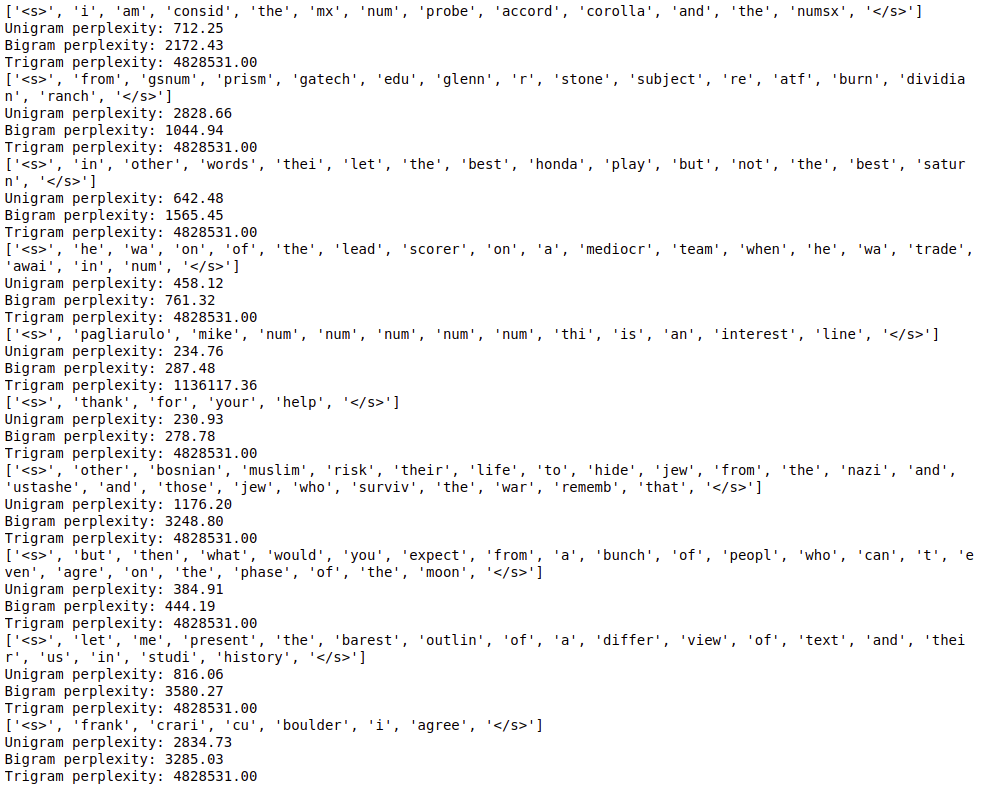
\includegraphics[width=\textwidth]{doc/images/perplexity.png}
    \caption{Cálculo de la perplejidad para distintas oraciones con diferentes modelos de lenguaje.}
    \label{fig:perplexity_sentences}
\end{figure}

Existen dos alternativas para solucionar esta situación y mejorar la calidad de los modelos de lenguaje: aumentar el tamaño del corpus ó disminuir el tamaño del vocabulario. Dado que aumentar el tamaño del corpus no es viable dada la antigüedad de los conjuntos de datos, se debería proceder a disminuir el vocabulario de los mismos. Un factor a tener en cuenta es que debido a los requerimientos del enunciado, no se eliminaron las palabras de parada (\textit{stopwords}). Una opción viable para este caso sería eliminar las palabras de parada, con lo cual se reduciría el tamaño del vocabulario. Otra alternativa sería la incorporación de más etapas de preprocesamiento de los datos con el fin de reducir el tamaño del vocabulario.


\section{\textit{Naive Bayes and Logistic Regression}}
\section{Análisis de sentimientos}
Para la tarea de análisis de sentimientos se utilizó una base de datos que contiene críticas realizadas por compradores de diferentes tipos de productos de cocina, películas, electrodomésticos y libros. Las reseñas contienen información del usuario que las escribió, ubicación, una calificación para diferentes aspectos como utilidad, ajuste del título, entre otros y finalmente un texto describiendo su opinión de la compra. Las reseñas están separadas en dos clases, positivas y negativas, y por lo tanto dos archivos. Adicionalmente hay un tercer archivo que contiene reseñas para hacer pruebas. A pesar de que el archivo se llama "sin etiqueta" vienen etiquetadas.

\subsection{Procesamiento de la base de datos}

Para el procesamiento de datos se utilizan los archivos llamados \textit{procesados}, por instrucción del profesor. En estos archivos cada línea de texto contiene únicamente las palabras encontradas en las reseñas y su frecuencia asociada, correspondiente a la cantidad de veces que aparecen en esa reseña y al final su etiqueta correspondiente: \textit{positive} o \textit{negative}.\\

Con esto en mente se recorren los archivos buscando generar un diccionario recopilando el todas las palabras que aparecen y almacenando un diccionario por cada reseña con la palabra y las repeticiones que tiene. Esto genero un diccionario de gran tamaño (>190.000 en el caso de la categoría 'libros'), razón por la cual se decidió verificar cuántas palabras tenían frecuencia unitaria una vez construido el \textit{dataset} de cada categoría. Esto mostró que más de 75\% del diccionario correspondía a palabras que aparecían únicamente en una reseña. Con base en esto se procedió a remover estas palabras resultando en un diccionario de menor tamaño. Cabe resaltar que para este vocabulario se utilizaron únicamente palabras del los archivos positivo y negativo, mas no del "sin etiquetas".\\

Con base en el diccionario obtenido para cada categoría se crean dos matrices de tamaño \textit{mxn} donde m corresponde al número de documentos y n al número de palabras del diccionario + 1 (correspondiente a la etiqueta asociada). En la primera matriz se almacena para cada documento la cantidad de veces que contiene cada palabra, constituyendo así el modelo BOW de cada documento. En la segunda matriz se almacena únicamente el hecho de que tenga o no la palabra, generando el modelo BOW booleano. De igual manera, se realiza el proceso para los archivos sin etiqueta obteniendo así seis matrices que se almacenan haciendo uso de la función \url{np.save()} de \textit{NumPy}.\\

En el caso de la unión de todas las categorías se realiza la unión de todos los diccionarios manteniendo únicamente una repetición de cada palabra. Esto genera una diccionario de 100.000 palabras, con base en el cual se realiza el mismo procedimiento previamente mencionado. Se obtienen entonces otras seis matrices de mayor tamaño conteniendo toda la base de datos completa.\\

Ahora bien, para el proceso de extracción de características con base en lexicones se realizo una investigación de cuáles son las características más utilizadas para este tipo de análisis. En \cite{Paper_lexicones} destacan que las principales características que se pueden extraer son \textit{i)} número de palabras positivas \textit{ii)} número de palabras negativas \textit{iii)} palabras positivas divido entre palabras negativas \textit{iv)} polaridad de la última palabra \textit{v)} suma de puntaje de palabras positivas y \textit{vi)} suma de puntaje de palabras negativas. Con esto en mente, se analiza qué información se puede extraer de cada lexicón ofrecido por el profesor resultando en las siguientes características:

\begin{itemize}
    \item Número de palabras positivas de acuerdo con SentiWordNet.
    \item Número de palabras negativas de acuerdo con SentiWordNet.
    \item Total de palabras positivas entre total de palabras negativas.
    \item Polaridad de la última palabra.
    \item Suma de puntajes de palabras negativas.
    \item Suma de puntajes de palabras positivas.
    \item Número de palabras negativas de acuerdo con ANFII.
    \item Número de palabras positivas de acuerdo con ANFII.
    \item Puntaje de palabras negativas.
    \item Puntaje de palabras positivas.
    \item Número de palabras positivas de acuerdo con WordStat.
    \item Número de palabras negativas de acuerdo con WordStat.
    \item Suma de polaridad de las palabras de acuerdo con Senticnet.
\end{itemize}

Esta extracción resulta entonces en una matriz donde las columnas (catorce) corresponden a las características previamente listadas más la etiqueta y las filas corresponden a documentos de los cuales se extrajo la información. Teniendo en cuenta que las características de lexicones no está ligas al \textit{dataset}, la matriz conjunta de todas las categorías se construye juntando las de cada categoría independientemente.

\subsection{Clasificadores}
Para el entrenamiento y comparación de los clasificadores se crea una función que recibe por parámetro un tipo de clasificador que puede ser Regresión Logística (LR), Naive Bayes (NB), Árbol de decisión (DT) o \textit{Random Forest} (RF), un dataset, que puede ser \textit{books}, \textit{dvd}, \textit{kitchen}, \textit{electronics} y \textit{all} y un modelo, que puede ser \textit{bow}, \textit{bool-bow} o \textit{lexicon}. Se utiliza la función \url{train\_test\_split()} de \textit{sklearn}  para obtener datasets separados para entrenamiento (80\%) y validación (20\%). Con estos parámetros se procede a cargar el archivo correspondiente al dataset y modelo indicado y posteriormente a entrenar el clasificador indicado.\\

Este entrenamiento se realiza utilizando la librería \textit{sklearn} de \textit{Python} con los parámetros predeterminados para cada uno de los clasificadores. Posteriormente, se realiza una predicción sobre los datos de validación y con esta se mide \textit{accuracy}, \textit{precision}, \textit{recall} y \textit{f1-score}, nuevamente utilizando la librería \textit{sklearn}. Todos estos valores se almacenan en un DataFrame de pandas para facilitar su comparación.\\

En caso de recibir como parámetro \textit{dataset == all} se utilizan los archivos que contienen todas las categorías mezcladas. A continuación, se comparan los resultados obtenidos.

\subsubsection{Comparación}
Como se indica en las instrucciones de la tarea, se evalúan las cuatro métricas más comunes para medir el desempeño cada uno de los modelos. El resultado de cada métrica se almacena en un DataFrame mostrado a continuación (\textit{véase tabla} \ref{tag:SAresults}). Allí se muestra para cada entrenamiento el \textit{dataset} que se utilizó, el clasificador seleccionado, el modelo escogido y el valor resultante de todas las métricas aplicadas.

\input{resources/SA-df.txt}

Lo anterior muestra claramente que el desempeño en general de todos los modelos es muy similar. No hay un modelo que sobresalga en todas las métricas. A continuación, se muestran promedios de los resultados agrupando para cada parámetro.

\begin{figure}[H]
    \centering
    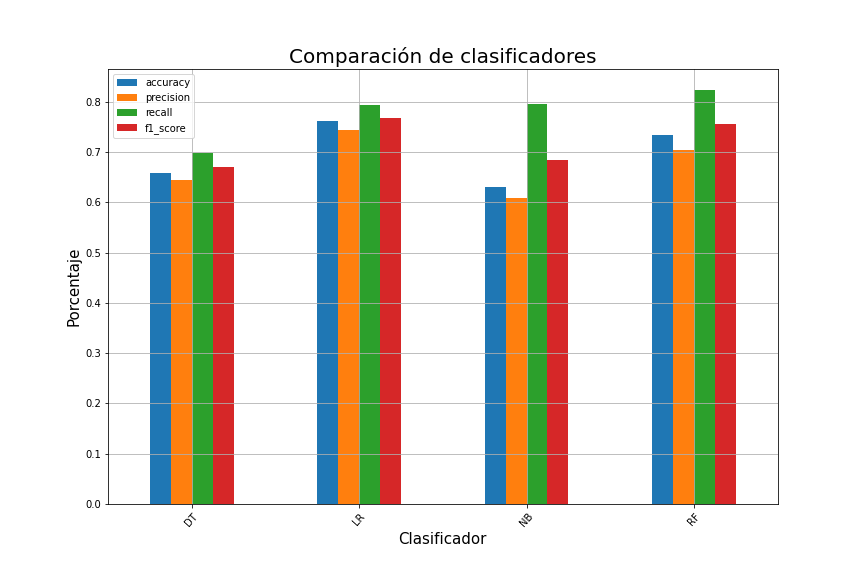
\includegraphics[scale = 0.45]{results/classifier_comparison.png}
    \caption{Comparación de clasificadores}
    \label{fig:classifier_comparisson}
\end{figure}

En la figura \ref{fig:classifier_comparisson} se puede ver el promedio de desempeño de cada uno de los clasificadores probados para cumplir con la tarea de análisis de sentimientos. Se hace evidente que el resultado del árbol de decisión y Naive Bayes son ligeramente inferiores a los demás, con un desempeño promedio de 0.65 y 0.72 respectivamente entre las métricas evaluadas. Esto es ligeramente mejor que adivinar, pues la probabilidad esperada de adivinar correctamente la clase es de 0.50.\\

En contraste los otros dos clasificadores (RF y LR) tienen un desempeño similar, resaltando que el mejor \textit{recall} corresponde a \textit{Random Forest} pero el mejor \textit{precision} corresponde a regresión logística. No obstante, dado que el \textit{recall} de LR es más alto, podría decirse que es el clasificador que mejor clasifica este dataset. 

\begin{figure}[H]
    \centering
    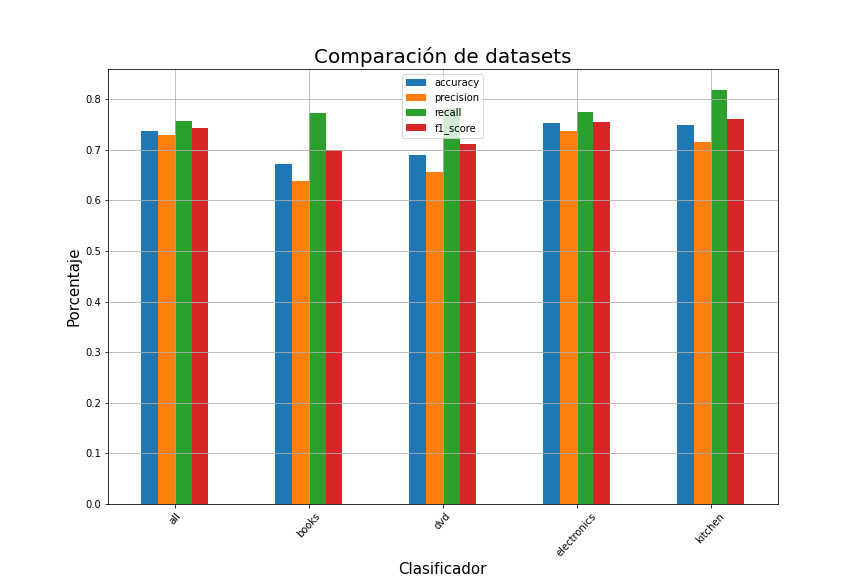
\includegraphics[scale = 0.45]{results/datasets_comparison.png}
    \caption{Comparación de datasets}
    \label{fig:dataset_comparison}
\end{figure}

En cuanto a la comparación de datasets (\textit{véase figura \ref{fig:dataset_comparison}}) los resultados son relativamente similares. En donde hay muy buen \textit{recall} un \textit{precision} bajo compensa. Podría decirse que los datasets de libros y películas son un poco más difíciles de de clasificar, mientas que electrónicos, cocina y todos juntos son un poco más fáciles. Se resalta la poca variación en las métricas resultantes de los clasificadores con todos los \textit{dataset} juntos al igual que en el de electrónicos. Ahora bien, analizando si es preferible o no entrenar modelo para cada categoría o para todas en conjunto, se hace evidente que el rendimiento en general de todos los \textit{datasets} juntos es mejor que los demás. Adicionalmente, solo se requiere un modelo. No obstante, es pertinente resaltar que el tamaño de la matriz de características del dataset 'all' es mayor, pues corresponde a la unión de los diccionarios asociados a cada categoría.

\begin{figure}[H]
    \centering
    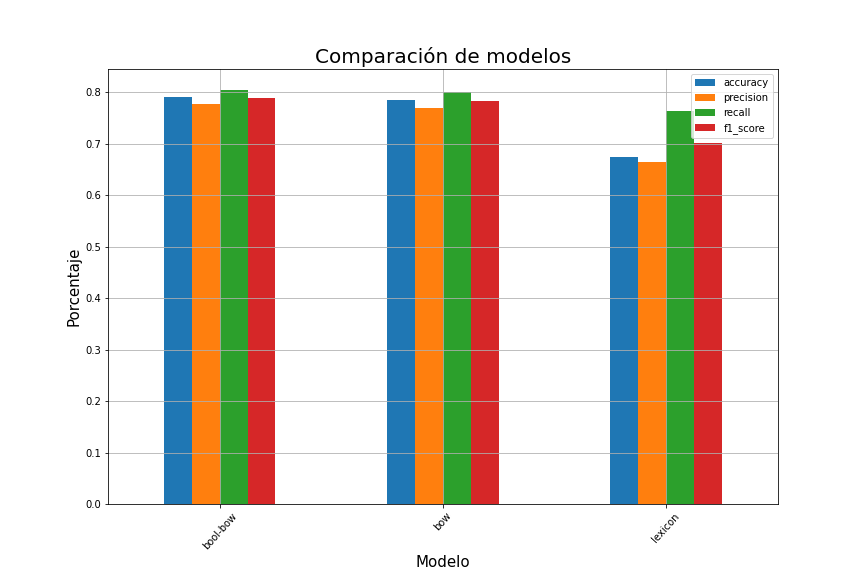
\includegraphics[scale = 0.45]{results/model_comparison.png}
    \caption{Comparación de modelos}
    \label{fig:model_comparisson}
\end{figure}

Ahora bien, los modelos de \textit{Bag of Words} booleano y no booleano tienen resultados casi que idénticos. Los resultados de los modelos de lexicones tienen resultados ligeramente menores, resaltando que \textit{recall} es bastante alto. Adicionalmente, la construcción de cada uno de los modelos no tiene mayor diferencia ni en tiempo ni en capacidad computacional requerida para ejecución o para entrenamiento de los modelos.

\textbf{Característica más importante para regresión logística}\\
Ahora bien, se desea verificar cuál es la característica más importarte para el clasificador de Regresión Logística. Para ello, se obtiene el vector de coeficientes asociado a cada uno de los clasificadores y se busca cuál es el mayor y por consiguiente a qué palabra o característica está asociado. Los resultados se muestran en la tabla \ref{tab:LR-features}.

% Please add the following required packages to your document preamble:
% \usepackage{multirow}
\begin{table}[]
\centering
\caption{Características más importantes para LR}
\label{tab:LR-features}
\begin{tabular}{|l|l|l|}
\hline
\textbf{Categoría}           & \textbf{Modelo} & \textbf{Característica}            \\ \hline
\multirow{3}{*}{Books}       & Bool-BOW        & \multirow{2}{*}{'excellent'}       \\ \cline{2-2}
                             & BOW             &                                    \\ \cline{2-3} 
                             & Lexicon         & \# of negative words  SentiWordNet \\ \hline
\multirow{3}{*}{DVD}         & Bool-BOW        & 'great'                            \\ \cline{2-3} 
                             & BOW             & 'excellent'                        \\ \cline{2-3} 
                             & Lexicon         & \# of negative words  SentiWordNet \\ \hline
\multirow{3}{*}{Electronics} & Bool-BOW        & 'great'                            \\ \cline{2-3} 
                             & BOW             & 'great'                            \\ \cline{2-3} 
                             & Lexicon         & \# of negative words  SentiWordNet \\ \hline
\multirow{3}{*}{Kitchen}     & Bool-BOW        & 'great'                            \\ \cline{2-3} 
                             & BOW             & 'great'                            \\ \cline{2-3} 
                             & Lexicon         & \# of negative words  SentiWordNet \\ \hline
\multirow{3}{*}{All}         & Bool-BOW        & 'excellent'                        \\ \cline{2-3} 
                             & BOW             & 'excellent'                        \\ \cline{2-3} 
                             & Lexicon         & \# of positive words ANFII         \\ \hline
\end{tabular}
\end{table}

\subsubsection{Variación de parámetros de Random Forest}
Se procede a hacer variación de parámetros para el modelo de Random Forest. Se utiliza RandomSearchCV, una función de Sklearn que permite hacer una variación de parámetros aleatoria. En esta función se define cuál es la métrica que se busca maximizar; en este caso se utilizan \textit{precison} y \textit{recall}. Se indica entonces, según recomendación de \cite{Sklearn-RF} que los parámetros a variar son \textit{n\_estimadores} que corresponde al número de estimadores, \textit{max\_features} que corresponde al método para obtener el número máximo de características a tener en cuenta, \textit{criterion} que corresponde al algoritmo a utilizar para el entrenamiento del árbol, \textit{max\_depth} que corresponde a la profundidad máxima del árbol y \textit{max\_leaf\_nodes} que indica el número máximo de nodos 'hojas' (\textit{véase descripción a continuación)}.\\

La variación de los resultados con diferentes parámetros es realmente mínima. Como se puede apreciar en el \textit{notebook} correspondiente. No obstante, los mejores resultados se ven al utilizar log2 como número máximo de características, lo cuál es respaldado por la teoría\cite{Sklearn-RF} en donde afirman que esta es la mejor escogencia para tareas de clasificación.

\subsubsection{Evaluación de los modelos}
Se selecciona entonces el mejor modelo para cada categoría y se evalúa su desempeño en el \textit{dataset} de evaluación. Los resultados se muestran en al tabla \ref{tab:model_eval}
\begin{table}[]
\centering
\caption{Evaluación de modelos}
\label{tab:model_eval}
\begin{tabular}{|l|l|l|l|l|l|}
\hline
\textbf{Categoría} & \textbf{Modelo}     & \textbf{Accuracy} & \textbf{Precision} & \textbf{Recall} & \textbf{F1-score} \\ \hline
Books              & Logistic regression & 0.828             & 0.825              & 0.838           & 0.832             \\ \hline
Kitchen            & Logistic regression & 0.874             & 0.875              & 0.871           & 0.873             \\ \hline
DVD                & Random Forest       & 0.808             & 0.781              & 0.861           & 0.819             \\ \hline
Electronics        & Logistic Regression & 0.863             & 0.861              & 0.869           & 0.865             \\ \hline
All                & Random Forest       & 0.843             & 0.858              & 0.823           & 0.840             \\ \hline
\end{tabular}
\end{table}

\subsection{\textit{Decision tree and random forests}}

A continuación, se realiza un investigación detallada en los modelos de clasificación de árbol de decisión y \textit{Random forest}. Para ello se responden las siguientes preguntas:
\begin{itemize}
    \item \textbf{¿Qué es un árbol de decisión y cómo funciona?}\\
    
    Los árboles de decisión corresponden a un método supervisado de clasificación y/o regresión de \textit{Machine Learning}. Usualmente, un árbol está constituido por nodos, ramas y hojas. En los nodos se evalúa el valor de cierto atributo o característica. Las ramas conectan nodos con otros nodos y con hojas. Las hojas son nodos terminales que predicen la clase o la distribución.\\
    Hay dos tipos de árboles de decisión: árboles de clasificación y árboles de regresión. Los primeros involucran datos discretos mientras que los segundos trabajan con datos continuos \cite{Sklearn-DT}. \\
    El funcionamiento se basa en iniciar con un nodo terminal que es en donde se sabrá la clase a la que pertenece la observación. Luego se selecciona un atributo de la observación y se analizan los posibles valores que puede tomar y la incidencia de dicho atributo en la clase seleccionada. Este proceso se sigue recursivamente hasta llegar un criterio de parada. En cada uno de los nodos se selecciona la mejor división según un determinado criterio, los cuales se muestran a continuación:
    \begin{equation}
        gini(v) = 1-\sum_{y \in L} p(y|v)^2
    \end{equation}
    \begin{equation}
        entropy(v) = -\sum_{y \in L} p(y|v) \cdot log(p(p|v))
    \end{equation}
    Para determinar qué tan bien se comporta una condición se compara el grado de impureza del nodo padre con el grado de impureza de los nodos hijos. Entre mayor sea la diferencia mejor resultaría dividir bajo esa condición.  
    
    \item \textbf{¿Cuál algoritmo se utiliza para construir un árbol de decisión?}\\
    
    A continuación se mencionan los principales algoritmos de entrenamiento de árboles de decisión. La información se obtiene de \cite{Sklearn-DT}.
    \begin{itemize}
        \item \textit{Iterative Dichotomiser 3:} El algoritmo crea un árbol con múltiples caminos evaluando para cada nodo cuál es la característica categórica que ofrece la mayor ganancia de información (information gain) para las etiquetas de clase. El árbol crece hacia abajo hasta alcanzar su tamaño máximo y se aplica una etapa de \textit{pruning} o poda. 
        \item \textit{C4.5:} Es el sucesor del algoritmo previamente descrito. Retira la condición de que las características deben ser categóricas definiendo dinámicamente atributos discretos que permiten partir el atributo continuo en diferentes sets de intervalos.
        \item \textit{C5.0:} Es una versión mejorada de C4.5 que utiliza menos memoria y crea sets de decisión más pequeños siendo más acertado. Está liberado bajo licencia de propiedad.
        \item \textit{\textbf{CART:}} Es similar a C4.5 pero soporta objetivos numéricos (regresión). Construye árboles binarios usando la característica que más ganancia de información ofrezca en cada nodo. Es el utilizado por \textit{scikit-learn}.
    \end{itemize}
    \item \textbf{¿Un árbol de decisión es un modelo generativo o discriminativo?}\\
    
    La diferencia fundamental entre un modelo discriminativo y uno generativo radica en que el modelo discriminativo se aprende las diferencias entre clases mientras que el generativo modela la distribución de las clases individuales. Por esto mismo los árboles de decisión son modelos discriminativos. A través de condicionales y reglas de decisión el árbol va decidiendo si una observación específica se encuentra dentro de una clase o de la otra. \cite{DvsG}.
    
    \item \textbf{¿Qué es un método agrupado en \textit{Machine Learning}?}\\
    
    Un método de aprendizaje agrupado o \textit{ensemble learning} hace referencia a cuando agrupan varios modelos base con el fin de obtener una predicción óptima. Resulta preferible confiar en varios modelos que en uno solo. Adicionalmente, utilizar un conjunto de modelos ocasiona que le modelo sea más resistente a \textit{overfitting}.\\
    Es necesario asegurarse de que los modelos utilizados en el conjunto son independientes. Esto puede garantizarse utilizando diferentes tipos de algoritmos (redes neuronales, regresión logística, árboles de decisión, SVMs, etc.) o entrenando un mismo modelo con diferentes datos. Se pueden utilizar diferentes técnicas para garantizar la independecia de estos sets de datos como \textit{bagging}, \textit{boosting}, \textit{stacking}, entre otros.  
    
    \item \textbf{¿Qué es \textit{bagging}?}\\
    
    \textit{Bootstrap aggregating} o \textit{B-agging} es un algoritmo utilizado para mejorar la estabilidad de conjuntos de modelos (\textit{ensembles}) tanto de regresión como de clasificación.\\
    El método consiste en muestrear con reemplazo el dataset original generando una nueva cantidad de sub-datasets que pueden tener observaciones duplicadas pero que de seguro tienen observaciones nuevas. Este método se conoce como \textit{Bootstrap}. La decisión final respeto a la etiqueta de la observación se obtiene usando \textit{Aggregation}. Se puede realizar con base en el total de salidas o en la probabilidad de las predicciones.
    
    \item \textbf{¿Qué es \textit{Random Forest} y cómo funciona?¿\textit{Random Forest} utiliza \textit{bagging}?}\\
    
    De manera general, \textit{Random Forest} corresponde a un conjunto de múltiples árboles de decisión buscando obtener una predicción más acertada y estable, usualmente entrenados utilizando \textit{bagging}. En la figura \ref{fig:RF} se muestra de mejor manera su procedimiento. Como se mencionó previamente es importante que los modelos (en este caso los árboles) sean independientes y tengan correlación muy baja. Es en este punto donde interviene el método de \textit{bagging}.\\
    
    \begin{figure}
        \centering
        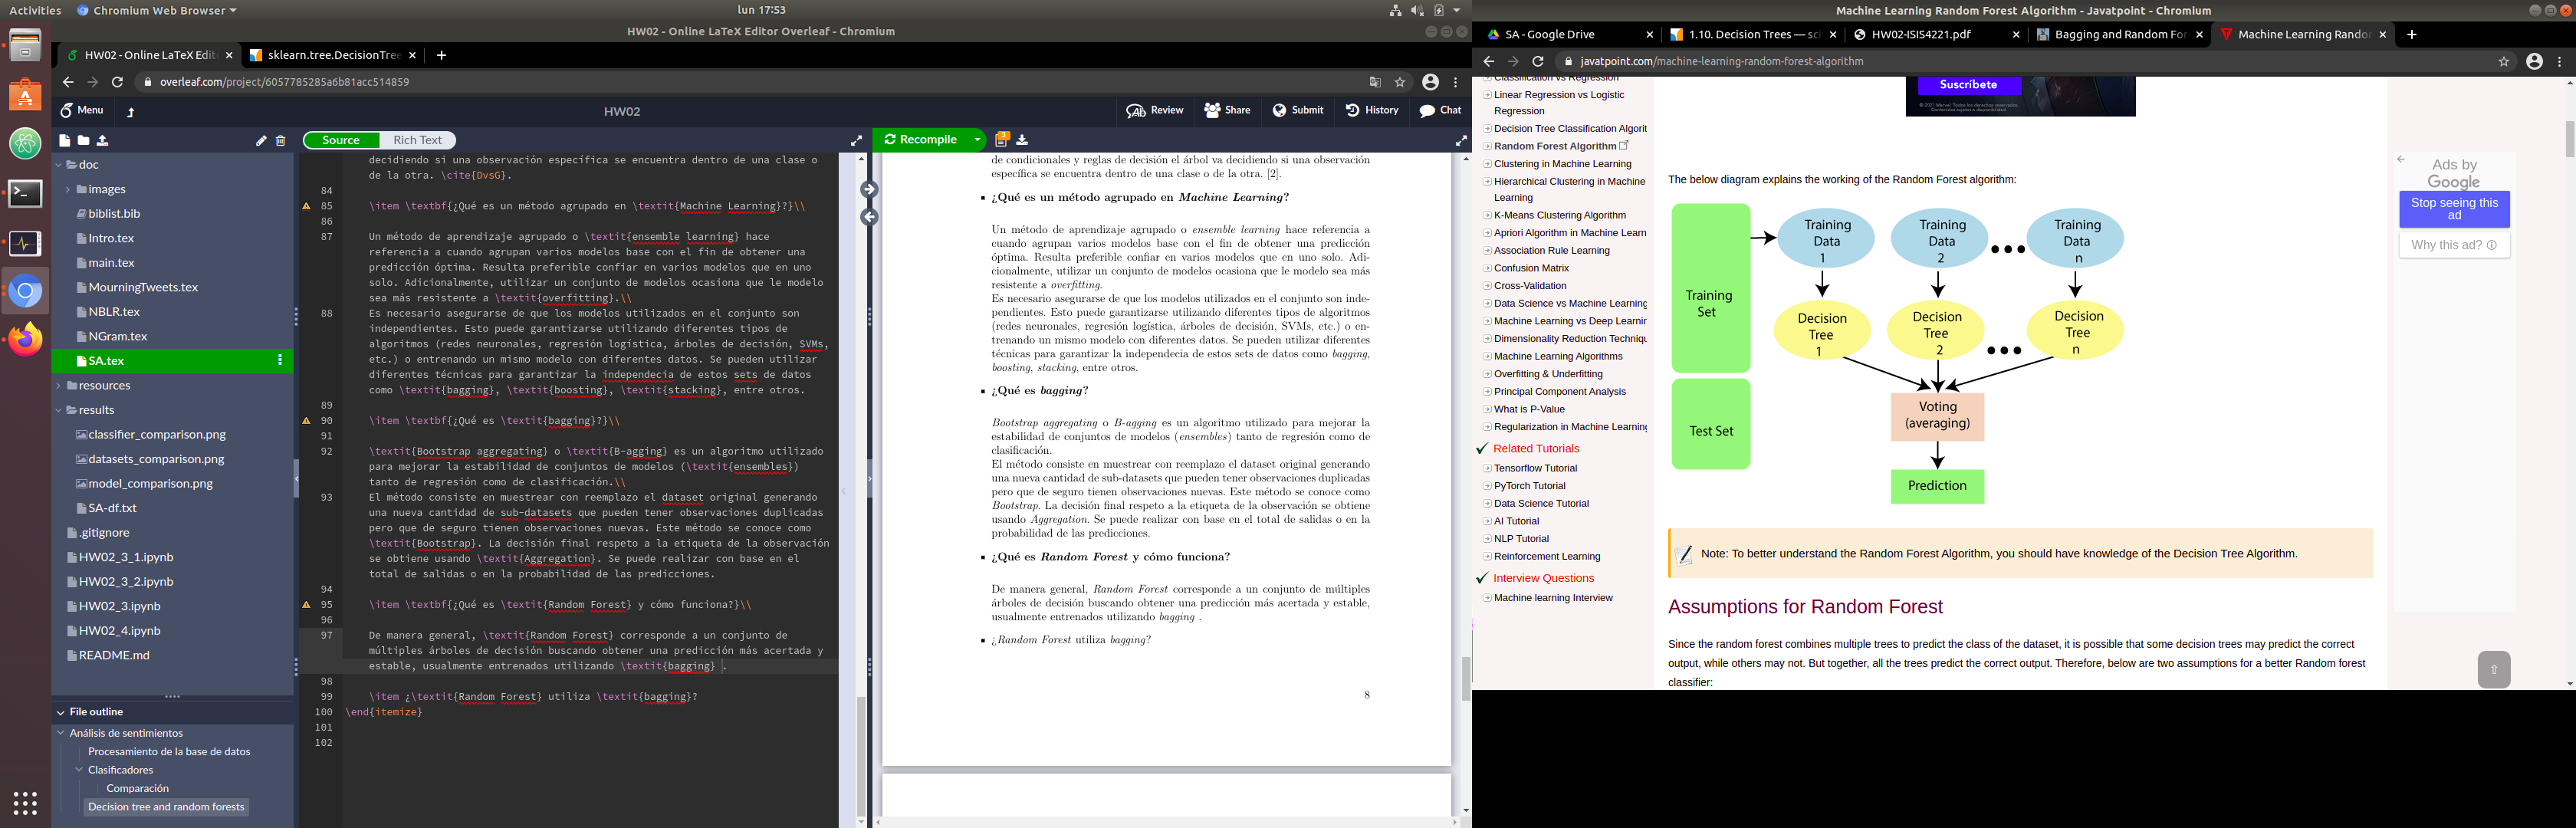
\includegraphics[trim={77cm 15cm 20cm 9cm}, clip, scale = 0.5]{doc/images/randomrofest.png}
        \caption{Random Forest (Tomado de \cite{javatpoint})}
        \label{fig:RF}
    \end{figure}
    
    Cabe resaltar que este algoritmo tiene ventajas en cuanto a que toma menos tiempo de entrenamiento comparado con otros, puede predecir con alto porcentaje de acierto y es capaz de mantener este porcentaje cuando hay una alta porción de datos faltantes \cite{javatpoint}.\\
    El proceso \cite{3} que sigue la creación de un \textit{Random Forest} se muestra a continuación:
    \begin{enumerate}
        \item Seleccionar aleatoriamente K observaciones del set de datos.
        \item Construir K árboles con diferentes set de entrenamiento.
        \item Votación de los K árboles con una observación. Para la votación en algoritmos tareas de clasificación se selecciona \textit{moda} y para regresión se utiliza \textit{media}.
        \item Seleccionar la clase o valor definitivo.
    \end{enumerate}
\end{itemize}


\newpage

\section{Mourning Tweets}

El desarrollo y código fuente de esta sección de la tarea se encuentra en el cuaderno \texttt{HW02\_4.ipynb} adjunto.

\subsection{Mourning Lexicon}

\subsubsection{Procesamiento de los \textit{Tweets}}

Antes de realizar la construcción de los \textit{Lexicones} e implementar los modelos de clasificación se realizó un proceso estándar para \textit{tokenizar} los \textit{tweets}. Para esto se hizo un procesamiento especial pensado en lenguaje especifico que se utiliza en \textit{Twitter} y las particularidades de ruido que este medio conlleva. Para esto se realizaron los siguientes pasos:

\begin{itemize}
    \item Remover la puntuación de los \textit{Tweets}.
    
    \item \textit{Tokenizar} el \textit{dataset} con el \textit{tokenizador} (\texttt{TweetTokenizer}) de \texttt{nltk} especializado para este tipo de datos. Esta herramienta:
    \begin{itemize}
        \item Estandariza todas las palabras a minúsculas.
        
        \item Reduce la longitud de las palabras en caso de repetir letras.
        
        \item Remueven caracteres especiales de \textit{Twitter} y usuarios (\textit{@}).
    \end{itemize}
    
    \item Remover las \textit{stop\_words} utilizando el set de palabras de \texttt{nltk} para cada uno de los idiomas (inglés y español).
    
    \item Con los términos (\textit{tokens}) de los \textit{tweets} se construye un vocabulario (o \textit{dictionary}) para cada uno de los \textit{datasets} (inglés y español). 
    
    \item Filtrar términos poco comunes (aquellos que aparecen en menos de 5 \textit{tweets}) y muy comunes (aquellos que aparecen en más del 75\% del \textit{dataset}). Para esto se uso la función \texttt{filter\_extremes} de \texttt{Gensim}. Esto resulto en vocabularios de alrededor de 5000 palabras para ambos idiomas.
    
\end{itemize}

\subsubsection{Construcción de lexicones}

Una vez se tienen definido el diccionario para los dos datasets, se construyen los lexicones estimando la probabilidad de que cada uno de los términos (\textit{tokens}) este en cada clase (luto o no luto). En este caso, la clase \textbf{luto \textit{(mourning)} se modela como la clase positiva} ($c = 1$) y la clase de \textbf{no luto \textit{(no mourning)} se modela como la clase negativa} ($c = 0$). \\

Para estimar dichas probabilidades, se utilizan los conceptos de verosimilitud  (\textit{likelihood}) y de verosimilitud escalada (\textit{scaled likelihood}). Las expresiones para dichas probabilidades son adaptadas de la referencia \cite{Potts2010SALT}, y se presentan a continuación:

\begin{equation}
    \mathbf{P(w|c=i)} = \frac{f(w,c=i)}{\sum_{w\in C} f(w,c=i)}
    \label{likelihood}
\end{equation} 

Al escalar esta probabilidadc condicional con las probabilidades \textit{a priori} de las palabras y las clases (utilizando el teorema de Bayes), se obtiene la siguiente probabilidad condicional:

\begin{equation}
    \mathbf{P(c=i|w)} = \frac{P(w|c=i) p(c=i)}{p(w)} = \frac{P(w|c=i)}{\sum_{c\in C} P(w|c=i)}
    \label{scaled_likelihood}
\end{equation} 

En \cite{Potts2010SALT}, sugieren trabajar con esta segunda probabilidad condicional pues un sentido más acorde. Dada la palabra, cual es la probabilidad que pertenezca a la clase. No obstante, para los dataset en cuestión se analizan ambas probabilidades.

\subsubsection{Resultados}
A partir de las expresiones (\ref{likelihood}) y (\ref{scaled_likelihood}), se calculan las probabilidades de cada termino para la clase mourning ($c=1$) en los dos datasets (inglés y español).

\begin{table}[H]
    \centering
    \caption{Resultado de los 15 términos con mayor probabilidad de aparecer en tweets de luto (\textit{mourning}) del \textit{dataset} en español (ES).}
    \label{tab:es_lexicons}
    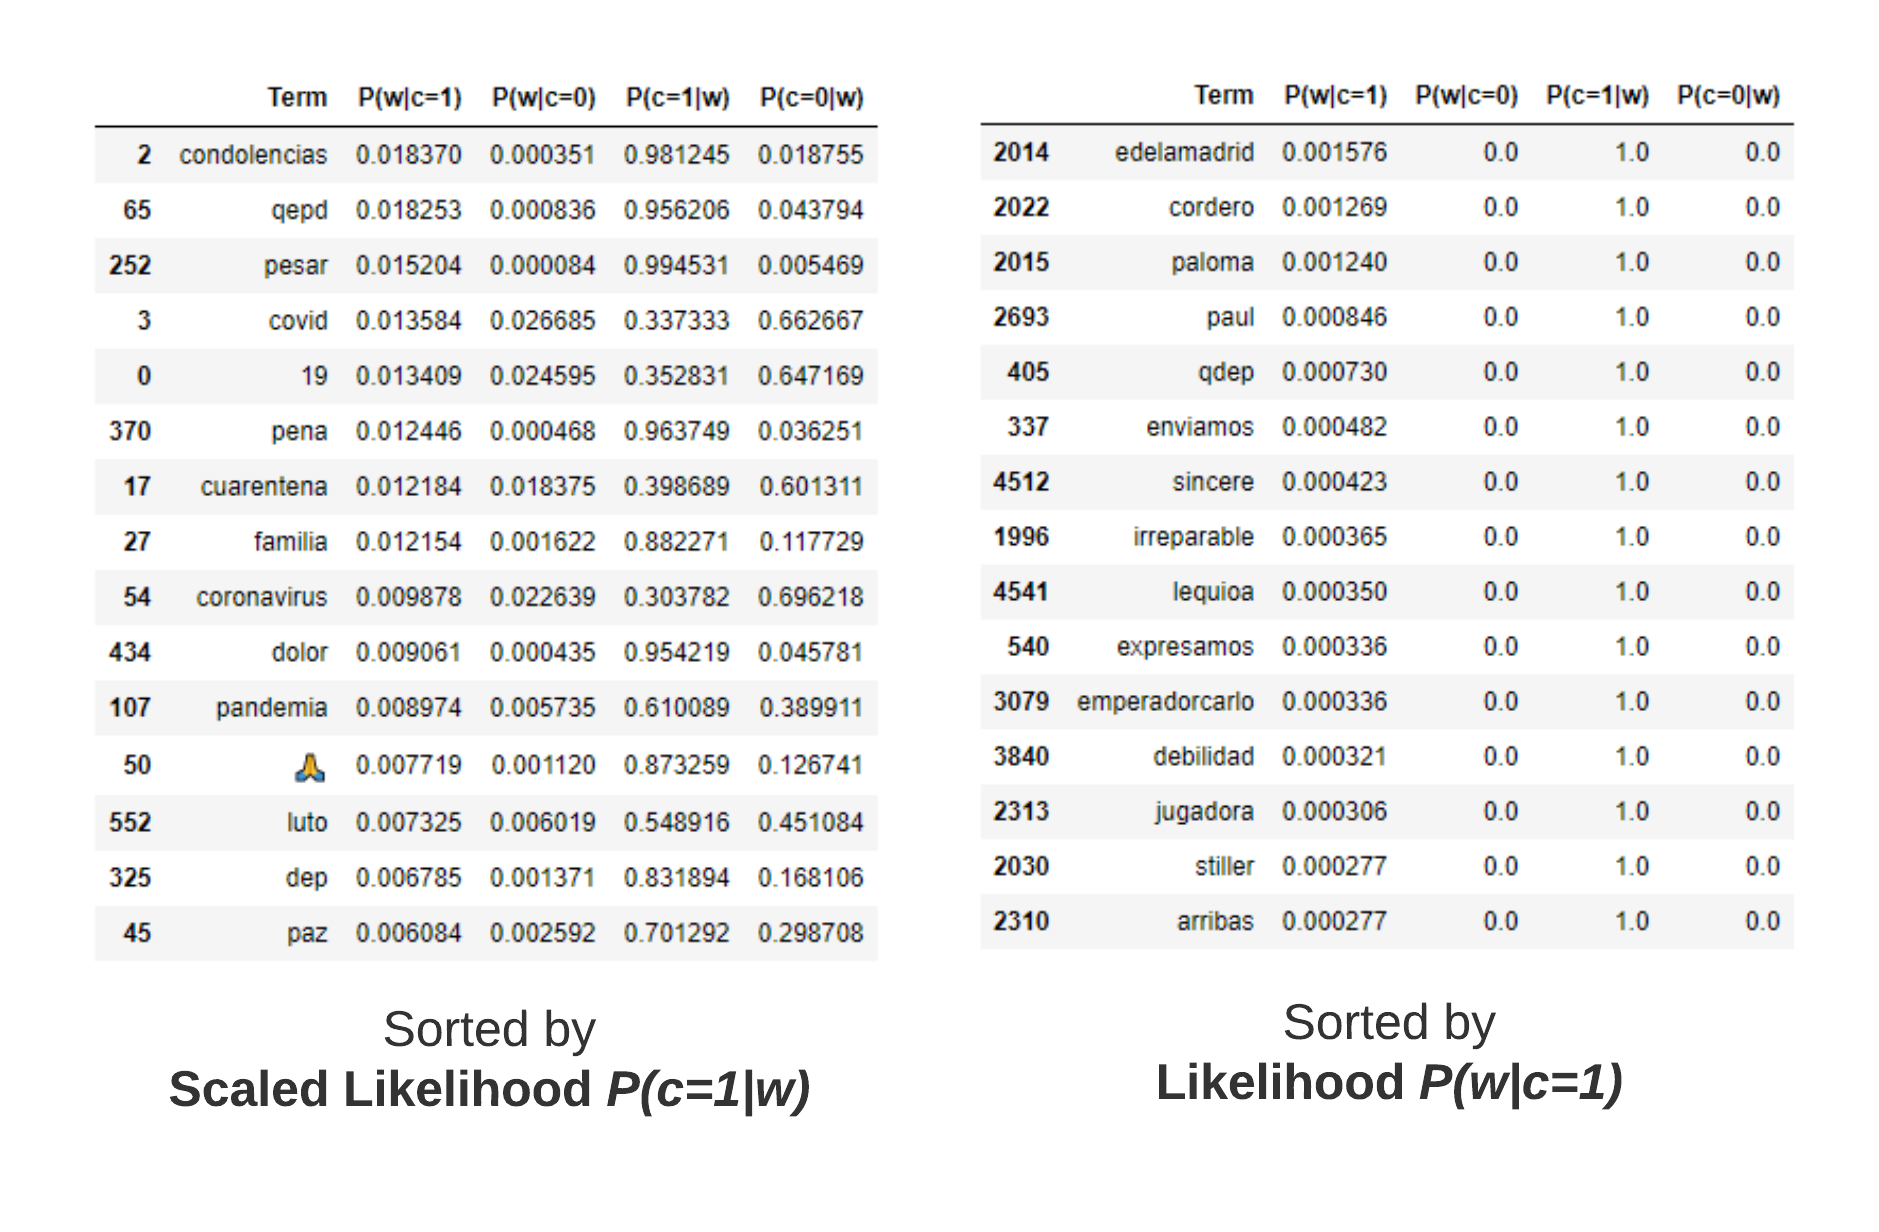
\includegraphics[width=\textwidth]{doc/images/ES_Lexicons.png}
\end{table}

\begin{table}[H]
    \centering
    \caption{Resultado de los 15 términos con mayor probabilidad de aparecer en tweets de luto (\textit{mourning}) del \textit{dataset} en inglés (EN).}
    \label{tab:en_lexicons}
    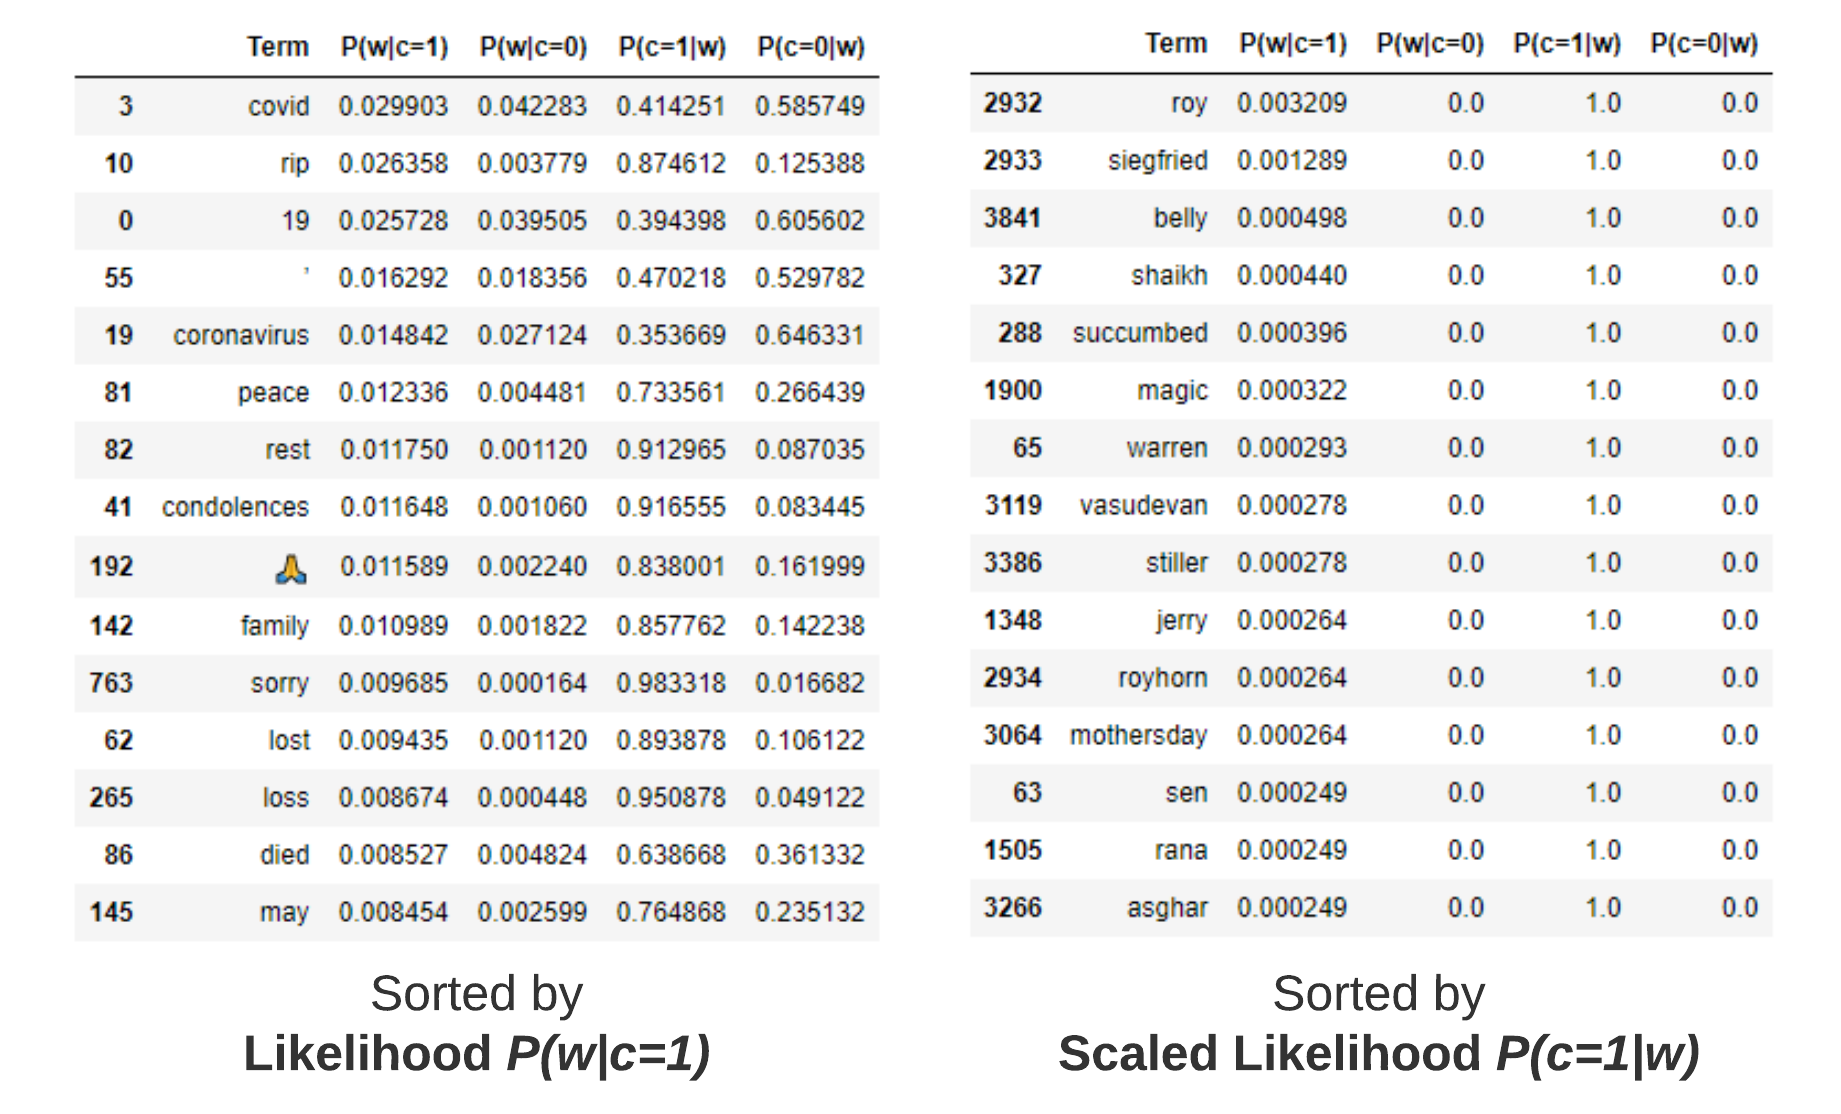
\includegraphics[width=\textwidth]{doc/images/EN_Lexicons.png}
\end{table}

En los cuadros \ref{tab:es_lexicons} y \ref{tab:en_lexicons} se observan los 15 términos con mayor probabilidad de pertenecer a un \textit{tweet} de luto para el \textit{dataset} en español y en inglés, respectivamente. En ambos casos se presentan los resultados ordenados tanto por su \textit{likelihood} (probabilidad $P(w|c=1)$) como por \textit{scaled likelihood} (probabilidad $P(c=1|w)$). En general los resultados son bastante similares en ambos idiomas, especialmente si se mira solo su probabilidad sin escalar. \\

En este caso, y a pesar de no estar ordenados exactamente igual, se observan términos muy similares en ambos idiomas. Acrónimos de luto como \textit{qdep}, el emoticón de las manos orando (id 50) y palabras como condolencias, pena, paz y familia (\textit{rip, condolences, peace, family, sorry}) se encuentran en ambas listas. De igual forma, al organizar los términos únicamente por esta probabilidad, se encuentran también palabras asociadas a la pandemia como coronavirus, covid, 19 en ambos idiomas. No obstante, es evidente que estos términos se encuentran ahí por su alta frecuencia a lo largo de todos los \textit{tweets}. Esto se puede afirmar poque, aunque su probabilidad condicional de pertenecer a la clase de luto $P(w|c=1)$ es muy alta, también lo es su probabilidad de pertenecer a la clase de no luto $P(w|c=0)$, e incluso en algunos casos es mayor. \\

Por otro lado, si se observan los términos ordenados por la probabilidad escalada $P(c=1|w)$ se obtiene una lista de palabras poco comunes. Esto se debe a que al escalar por la probabilidad de la palabra (dividir entre $p(w)$), las palabras poco comunes obtienen un peso muy importante. De hecho, el set de palabras que se obtiene, tiene en todos los términos la misma probabilidad (1). Esto quiere decir que son palabras que solo aparecen en la clase de luto (\textit{mourning}), a pesar de que su ocurrencia es realmente baja. 

\begin{table}[H]
    \centering
    \caption{Resultado de los 15 emoticones con mayor probabilidad de aparecer en tweets de luto (\textit{mourning}) del \textit{dataset} en español (ES).}
    \label{tab:es_emojis}
    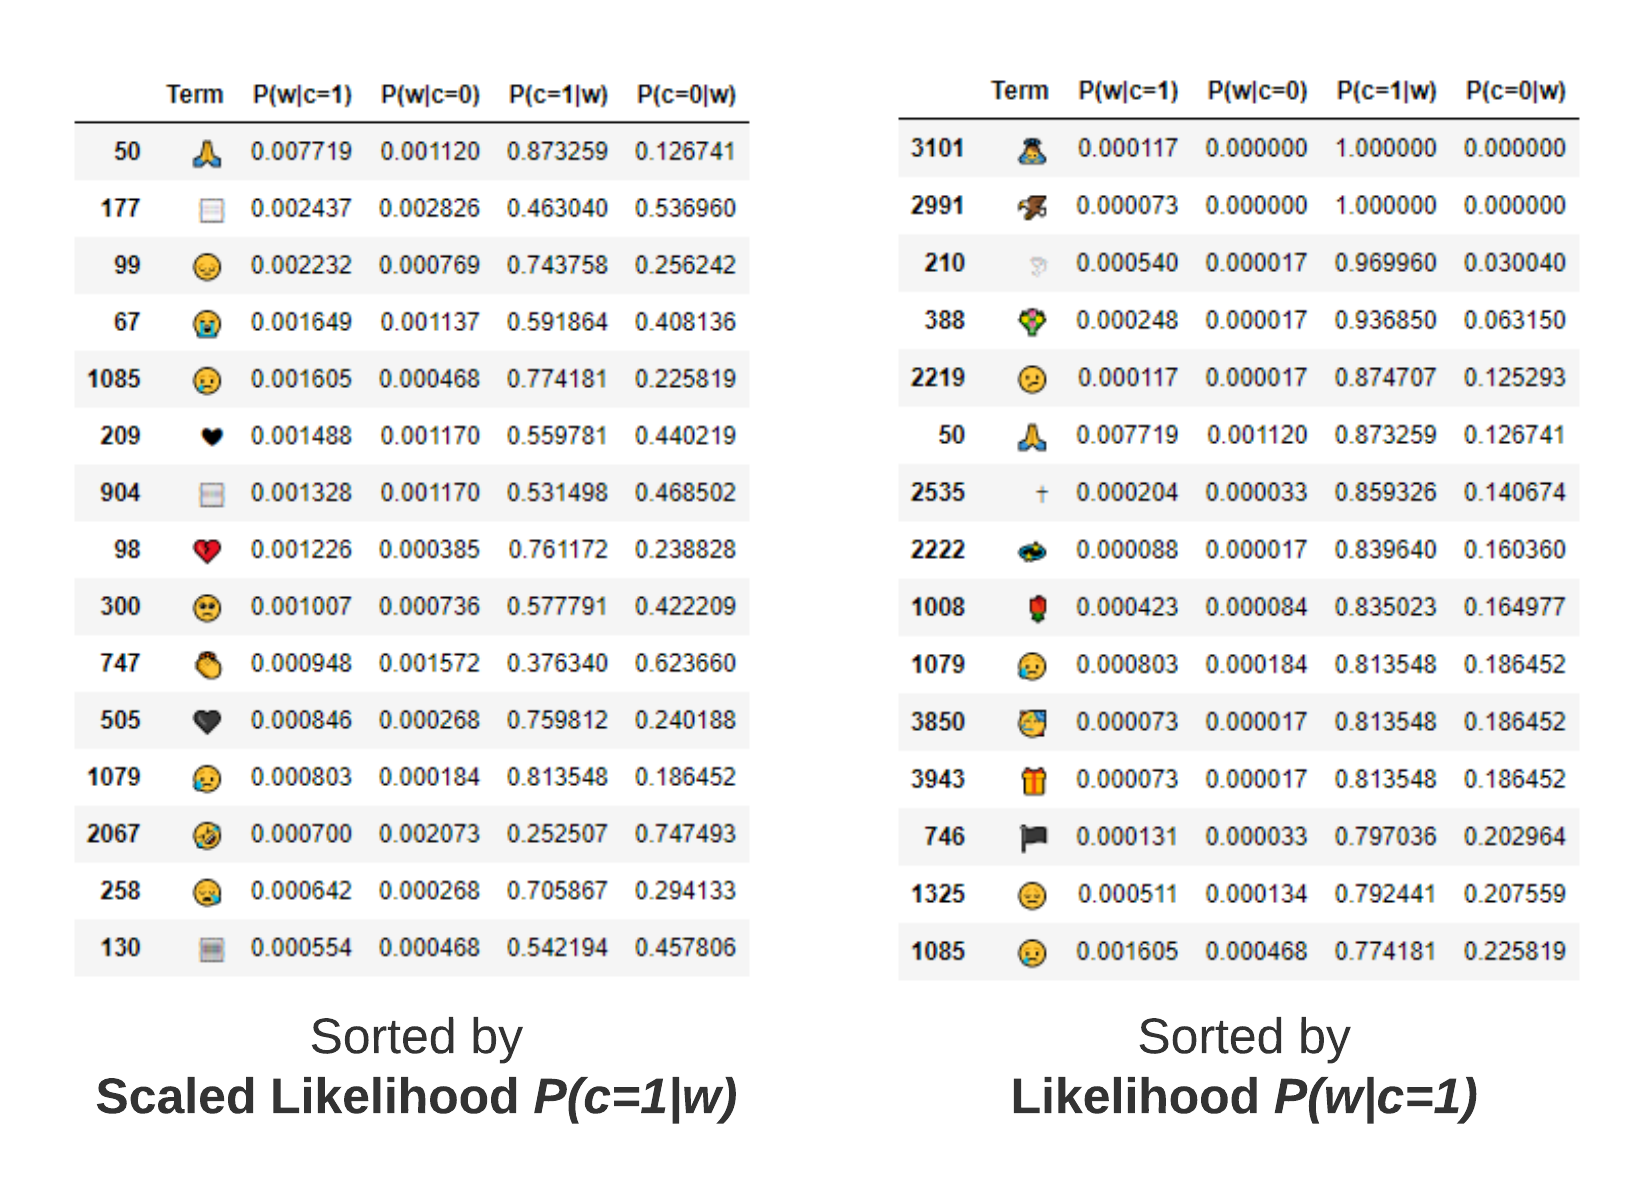
\includegraphics[width=\textwidth]{doc/images/ES_Emojis.png}
\end{table}

Ahora bien, algo similar a lo que ocurre con las palabras ocurre con los emoticones (véase cuadros \ref{tab:es_emojis} y \ref{tab:en_emojis}). Al mirar solo la lista ordenada por la probabilidad $P(w|c=1)$ se observan emoticones similares como: caritas tristes y llorando y corazones rotos y negros, en los \textit{datasets} de ambos idiomas. Adicionalmente, en ambos casos las manos orando encabezan la lista. No obstante, al ordenar por la probabilidad $P(c=1|w)$, se obtienen algunos emoticones poco comunes (como el guante de boxeo y el águila), cuya probabilidad es 1, pues solo aparecen en los \textit{tweets} de luto a pesar de su baja frecuencia. Sin embargo, empiezan a aparecer algunos otros con un sentido más relacionado al luto, como la paloma blanca, la cruz, un ángel y las flores. 

\begin{table}[H]
    \centering
    \caption{Resultado de los 15 emoticones con mayor probabilidad de aparecer en tweets de luto (\textit{mourning}) del \textit{dataset} en español (ES).}
    \label{tab:en_emojis}
    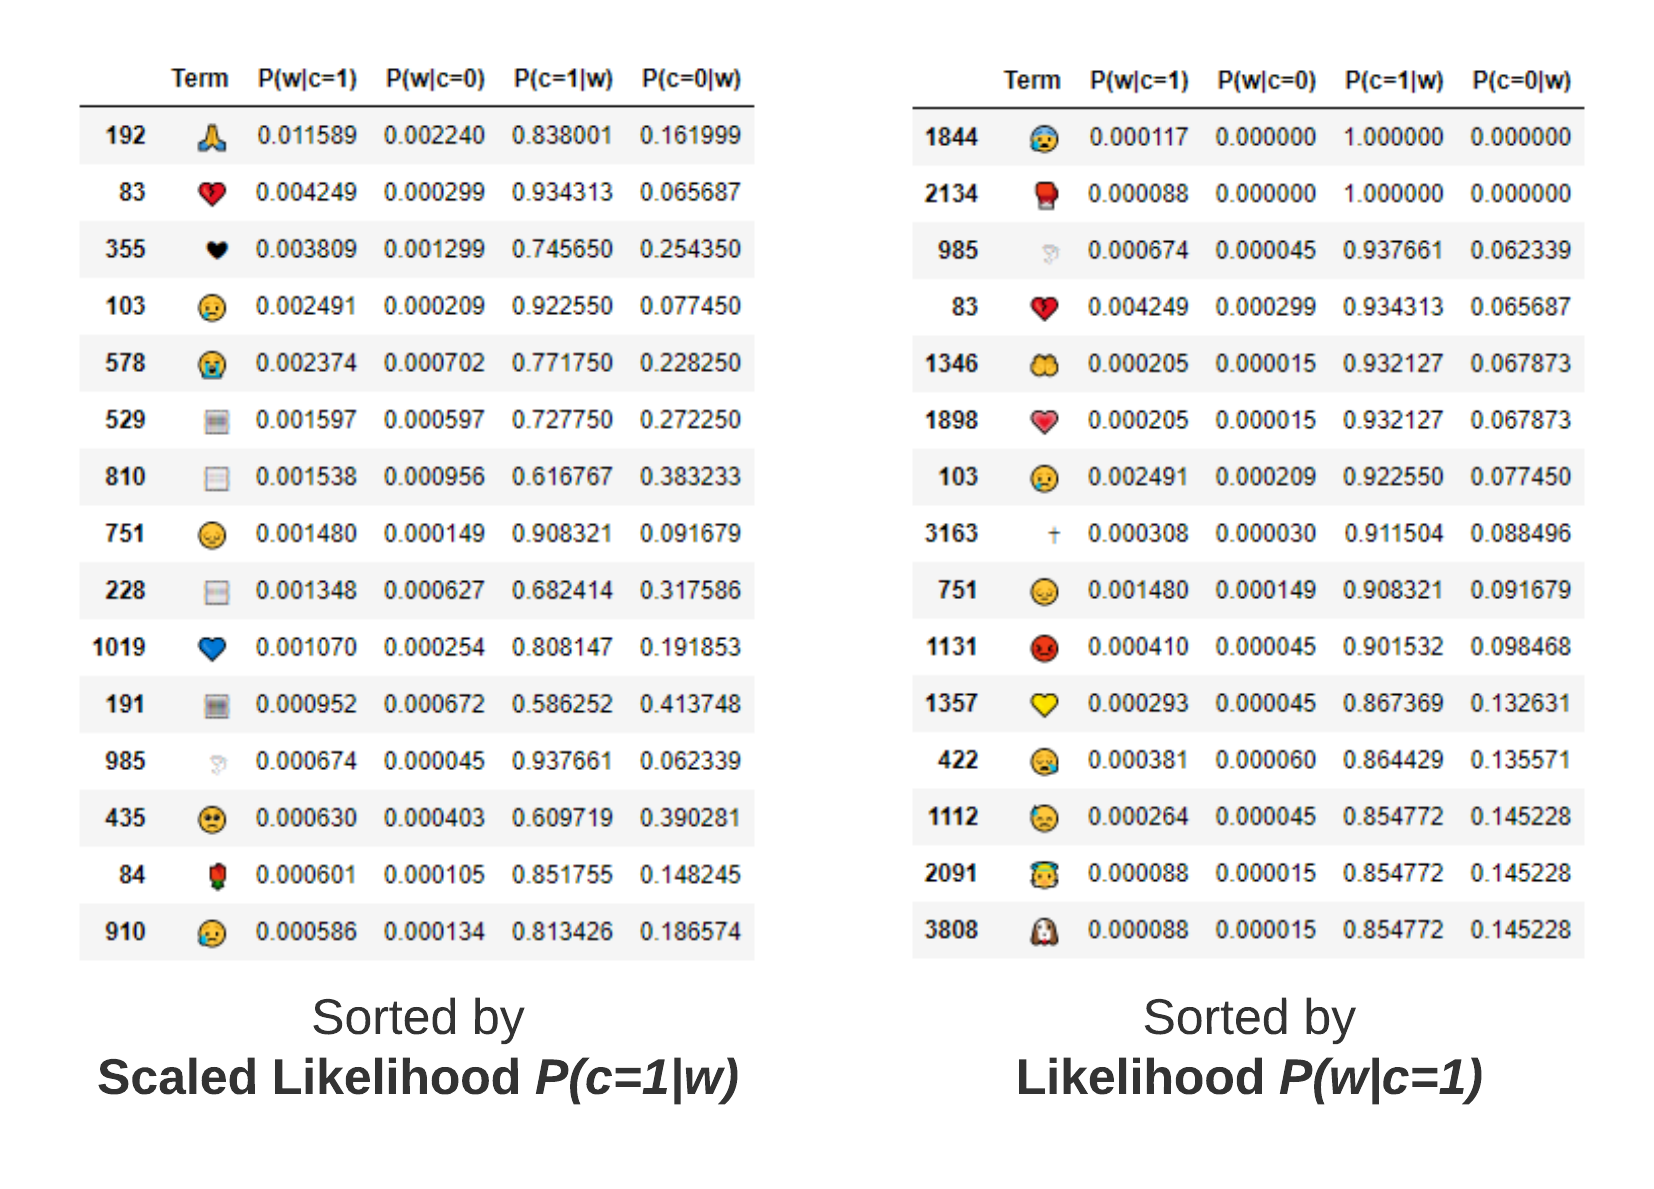
\includegraphics[width=\textwidth]{doc/images/EN_Emojis.png}
\end{table}

\subsection{Clasificadores}

\subsubsection{Representación de características}

Para poder entrenar un modelo de clasificación binario (clasificación de \textit{tweet} como luto o no luto) fue necesario convertir los \textit{tweets tokenizados} en un modelo de bolsa de palabras (\textit{BOW Model}). Esto permitirá después obtener información sobre los términos (\textit{tokens}) más relevantes para algunos de los modelos entrenados como clasificadores. \\

De igual forma, para poder evaluar el efecto de los emoticones (\textit{emojis}) en el entrenamiento, se construyeron dos representaciones de \textit{BOW}, una que los incluyera y otra que no. En total los emoticones (después del procesamiento de los \textit{tweets}) representaron aproximadamente un 3\% de los \textit{tokens} del vocabulario (alrededor de 150 términos en ambos idiomas). Por lo que el modelo BOW sin emoticones era de un tamaño ligeramente menor.

\subsection{Resultados}

Para entrenar los modelos se utilizó el 75\% de los datos y el resto del \textit{dataset} (25\%) se utilizó para poner a prueba el desempeño de los modelos presentado a continuación. En total se hicieron pruebas con 4 tipos de modelos (\textit{Naive Bayes, Logistic Regression, Decision Trees} y \textit{Random Forest}). Pero se entrenaron un total de 16 Modelos, dividendo las pruebas por idioma y por representación de caracteristicas (Modelos BOW que incluían o no los emoticones).

\begin{figure}[H]
    \centering
    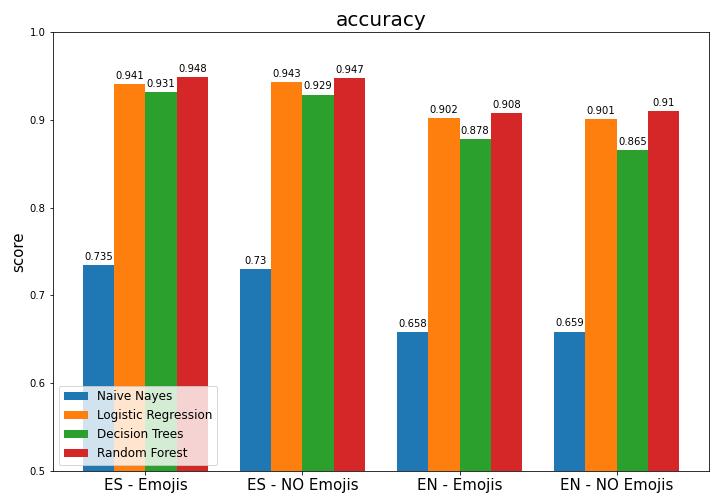
\includegraphics[width=0.8\textwidth]{results/mourning_tweets_accuracy.png}
    \caption{Resultados de \textit{Accuracy} para los distintos clasificadores sobre las distintas pruebas realizadas (\textit{datasets} en ingles y español y \textit{features} que incluyen o no \textit{emojis}.}
    \label{fig:mt_acc}
\end{figure}


\begin{figure}[H]
    \centering
    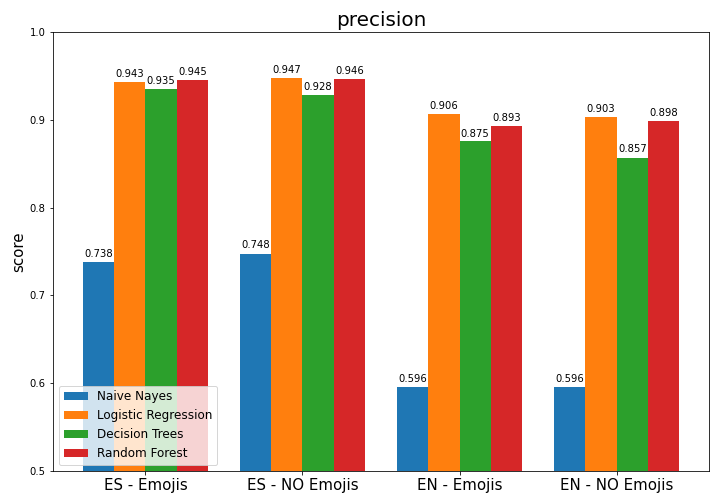
\includegraphics[width=0.8\textwidth]{results/mourning_tweets_precision.png}
    \caption{Resultados de \textit{Precision} para los distintos clasificadores sobre las distintas pruebas realizadas (\textit{datasets} en ingles y español y \textit{features} que incluyen o no \textit{emojis}.}
    \label{fig:mt_precision}
\end{figure}


\begin{figure}[H]
    \centering
    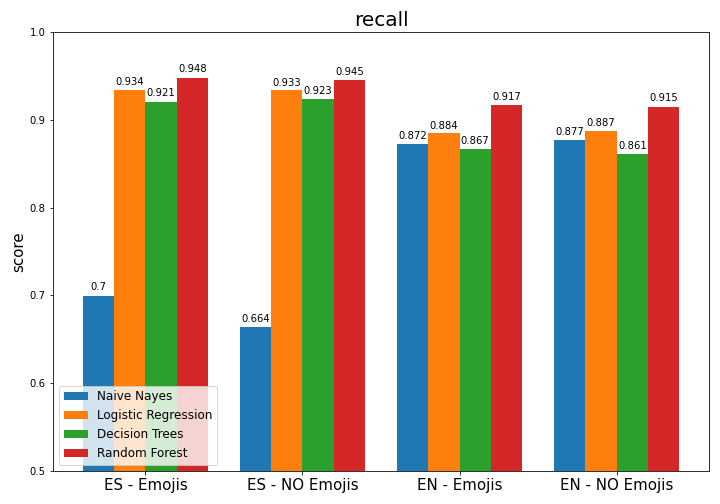
\includegraphics[width=0.8\textwidth]{results/mourning_tweets_recall.png}
    \caption{Resultados de \textit{Recall} para los distintos clasificadores sobre las distintas pruebas realizadas (\textit{datasets} en ingles y español y \textit{features} que incluyen o no \textit{emojis}.}
    \label{fig:mt_recall}
\end{figure}


\begin{figure}[H]
    \centering
    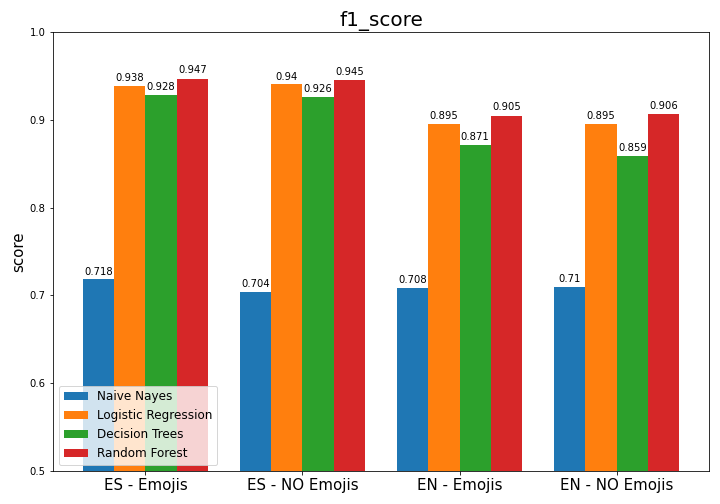
\includegraphics[width=0.8\textwidth]{results/mourning_tweets_f1_score.png}
    \caption{Resultados de \textit{F1 Score} para los distintos clasificadores sobre las distintas pruebas realizadas (\textit{datasets} en ingles y español y \textit{features} que incluyen o no \textit{emojis}.}
    \label{fig:mt_f1score}
\end{figure}

En términos generales se obtuvieron resultados bastante adecuados para una tarea de clasificación binaria. No obstante, que en todas las métricas el desempeño del clasificador de \textit{Naive Bayes} es considerablemente peor en todos los casos. Sin embargo, vale la pena destacar que su precisión aumenta bastante en el \textit{dataset} en español y su \textit{recall} aumenta considerablemente en el \textit{dataset} en inglés. \\

Por su parte los otros 3 clasificadores tienen desempeños bastante respetables, todos por encima del 90\% en casi todas las métricas. Siendo el \textit{Random Forest} el mejor clasificador, seguido del \textit{Logistic Regression} con un desempeño muy similar. Adicionalmente, también se puede observar que la tarea de clasificación fue ligeramente más difícil en inglés, pues en todos los casos se puede observar casi un 4\% de diferencia de desempeño en todas las métricas con el idioma español. En el cuadro \ref{tab:clf_summary} se puede observar un resumen de todos los resultados promedio obtenidos para cada uno de los clasificadores.


\begin{table}[H]
    \centering
    \caption{Resumen de resultados (métricas de desempeño) según clasificador y según idioma del \textit{dataset}}
    \label{tab:clf_summary}
    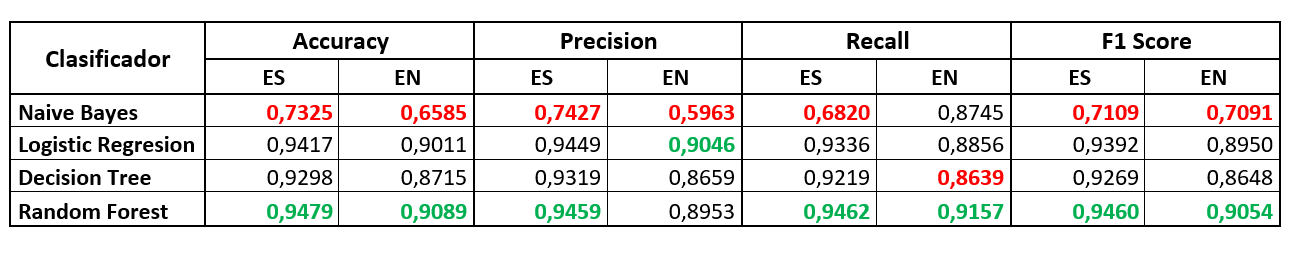
\includegraphics[width=\textwidth]{doc/images/summary_results_clf.png}
\end{table}

Ahora bien, en cuanto a la importancia de los emoticones, en el cuadro \ref{tab:emojis_summary} se puede observar el resultado promedio de todos los clasificadores agrupado por la inclusión o no de estos en su modelo de representación (\textit{BOW Model}). Aunque en casi todos los casos (salvo por la precisión en el idioma español) la inclusión de emoticones represento un mejor desempeño, en general la mejora es marginal y está lejos de ser categórica. Esto se puede deber al tamaño del \textit{dataset}, el cual es relativamente pequeño, pues aunque los emoticones brinden mayor información al problema, también pueden agregar un poco de ruido a la clasificación. No obstante, en términos generales se puede observar que su inclusión mejora el desempeño en ambos idiomas. 

\begin{table}[H]
    \centering
    \caption{Resumen de resultados (métricas de desempeño) según el \textit{set} de características (emojis o no emojis) utilizado para la clasificación y según el idioma.}
    \label{tab:emojis_summary}
    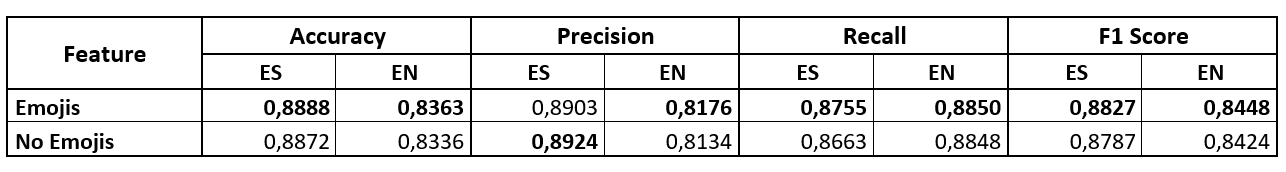
\includegraphics[width=\textwidth]{doc/images/summary_results_emoji.png}
\end{table}

\subsection{Análisis de importancia de características}

Finalmente, se desea evaluar que términos o emoticones son relevantes para la clasificación a partir de los modelos construidos. Esto con el fin de comparar estos resultados con los de los lexicones construidos anteriormente (véase literal 4.2). Para esto se evaluaron los parámetros de la regresión logística (LR) y del modelo de \textit{Random Forest} (RF). Los cuales se presentan a continuación

\subsubsection{Logistic Regression (LR)}

\begin{table}[H]
    \centering
    \caption{Términos con mayor peso dentro de los parámetros de Regresión Logística (LR) en el \textit{dataset} en español (ES)}
    \label{tab:lr_coef_es}
    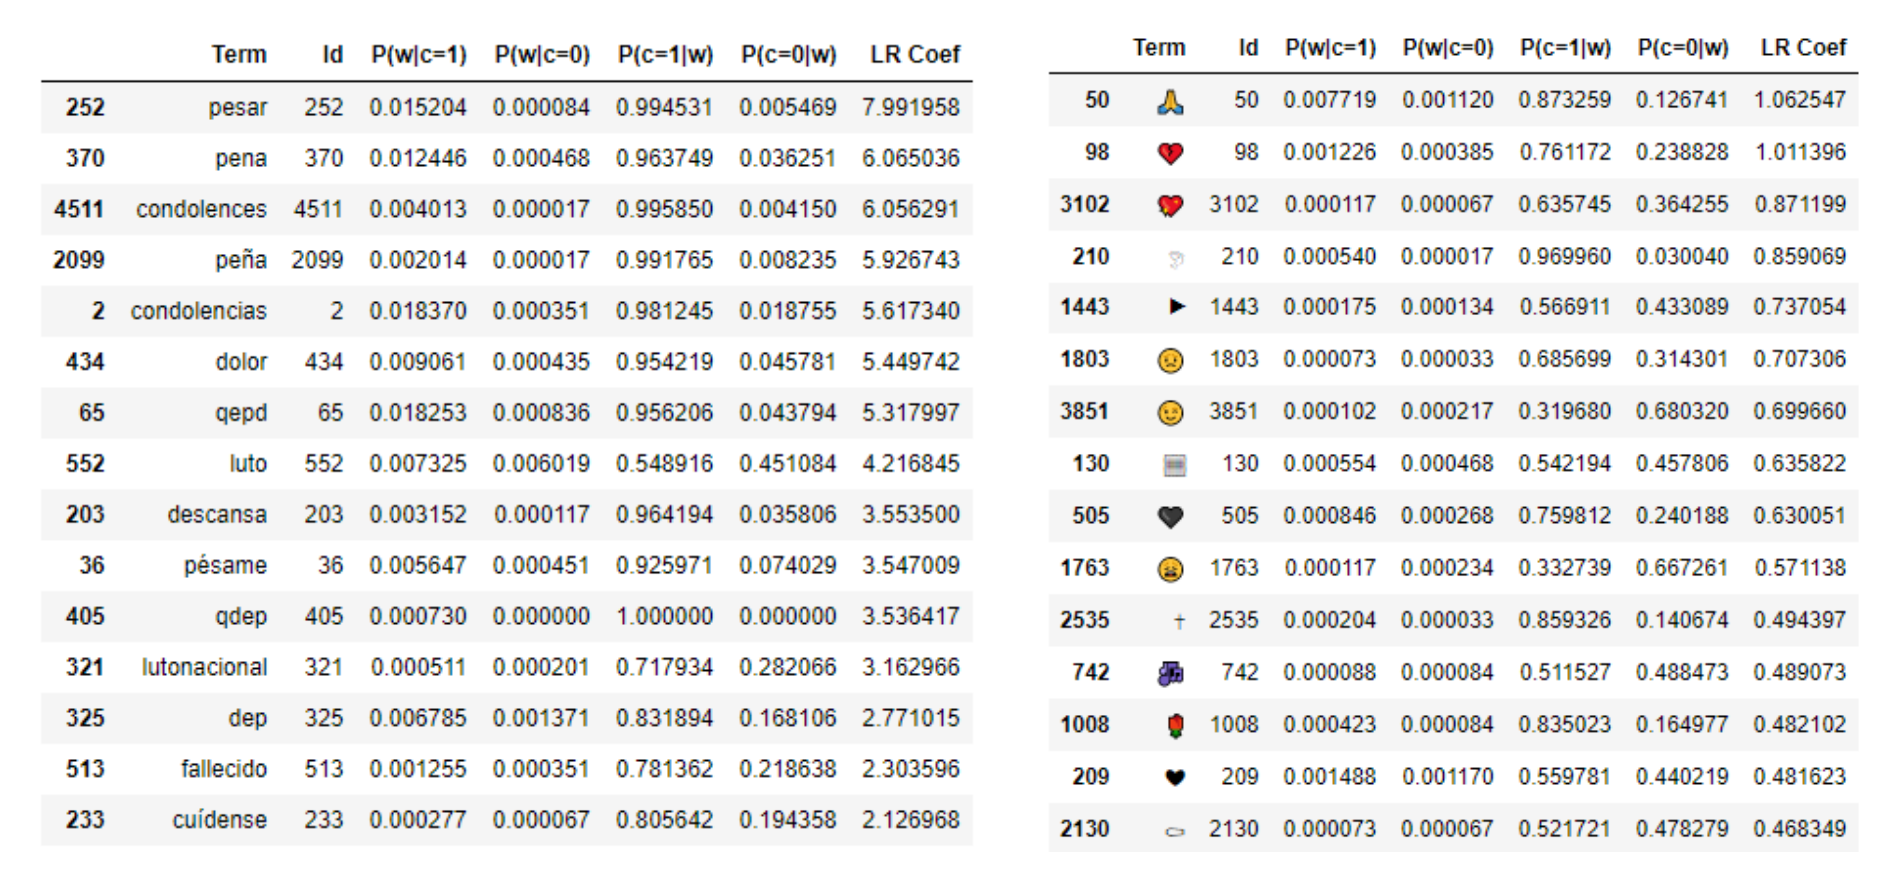
\includegraphics[width=\textwidth]{doc/images/LR_Coef_es.png}
\end{table}

\begin{table}[H]
    \centering
    \caption{Términos con mayor peso dentro de los parámetros de Regresión Logística (LR) en el \textit{dataset} en inglés (EN)}
    \label{tab:lr_coef_en}
    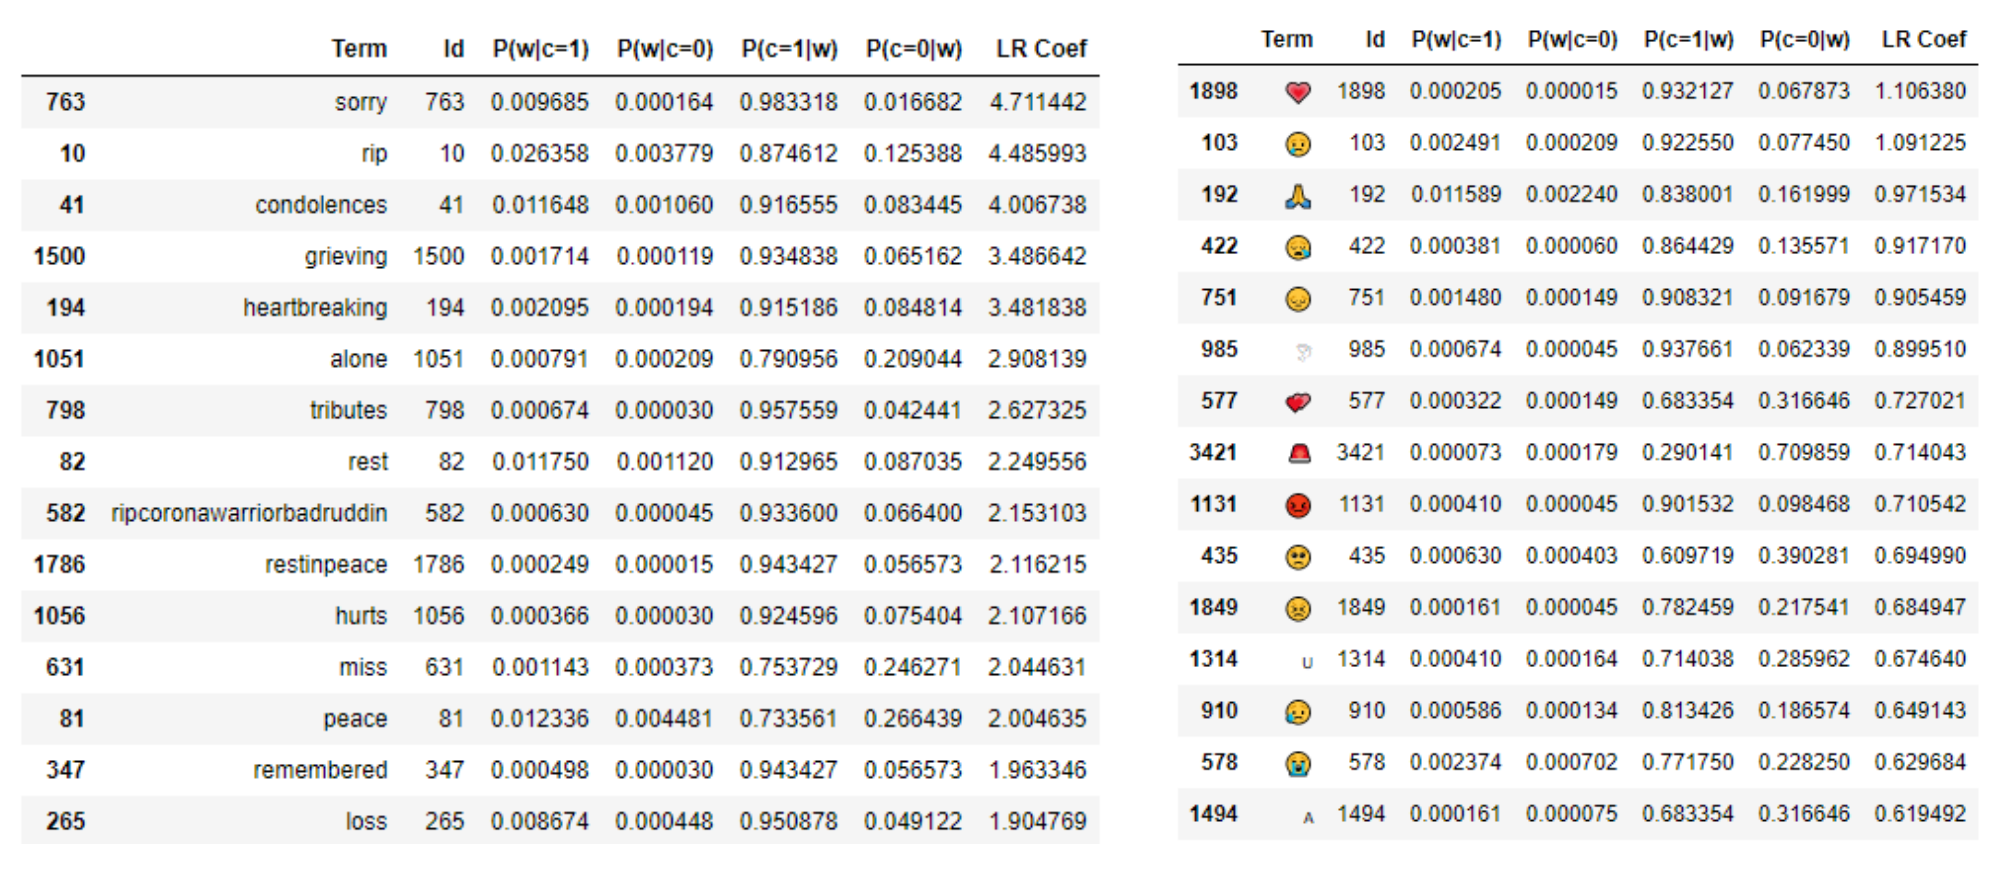
\includegraphics[width=\textwidth]{doc/images/LR_Coef_en.png}
\end{table}

\subsubsection{Random Forest (RF)}

\begin{table}[H]
    \centering
    \caption{Términos con mayor peso dentro de los parámetros de Random Forest (RF) en el \textit{dataset} en español (ES)}
    \label{tab:lr_coef_es}
    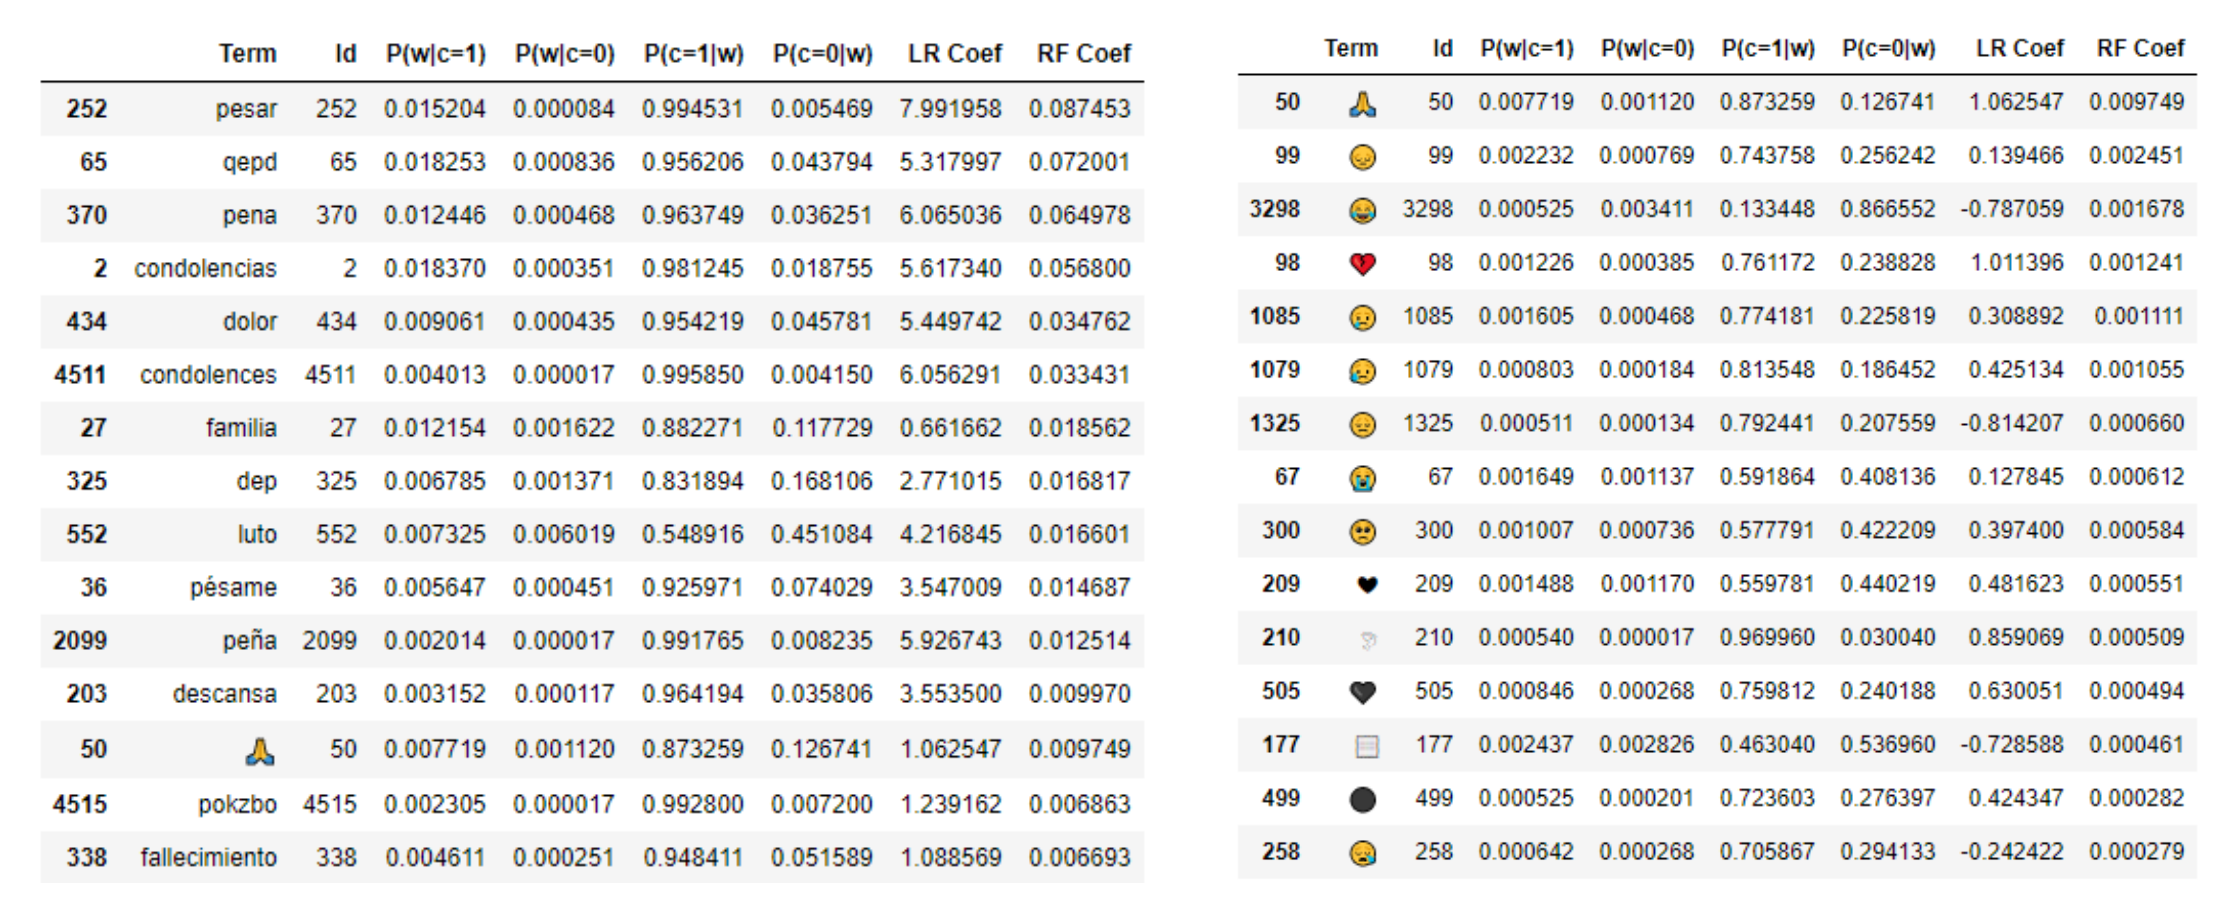
\includegraphics[width=\textwidth]{doc/images/RF_Coef_es.png}
\end{table}

\begin{table}[H]
    \centering
    \caption{Términos con mayor peso dentro de los parámetros de Random Forest (RF) en el \textit{dataset} en inglés (EN)}
    \label{tab:lr_coef_en}
    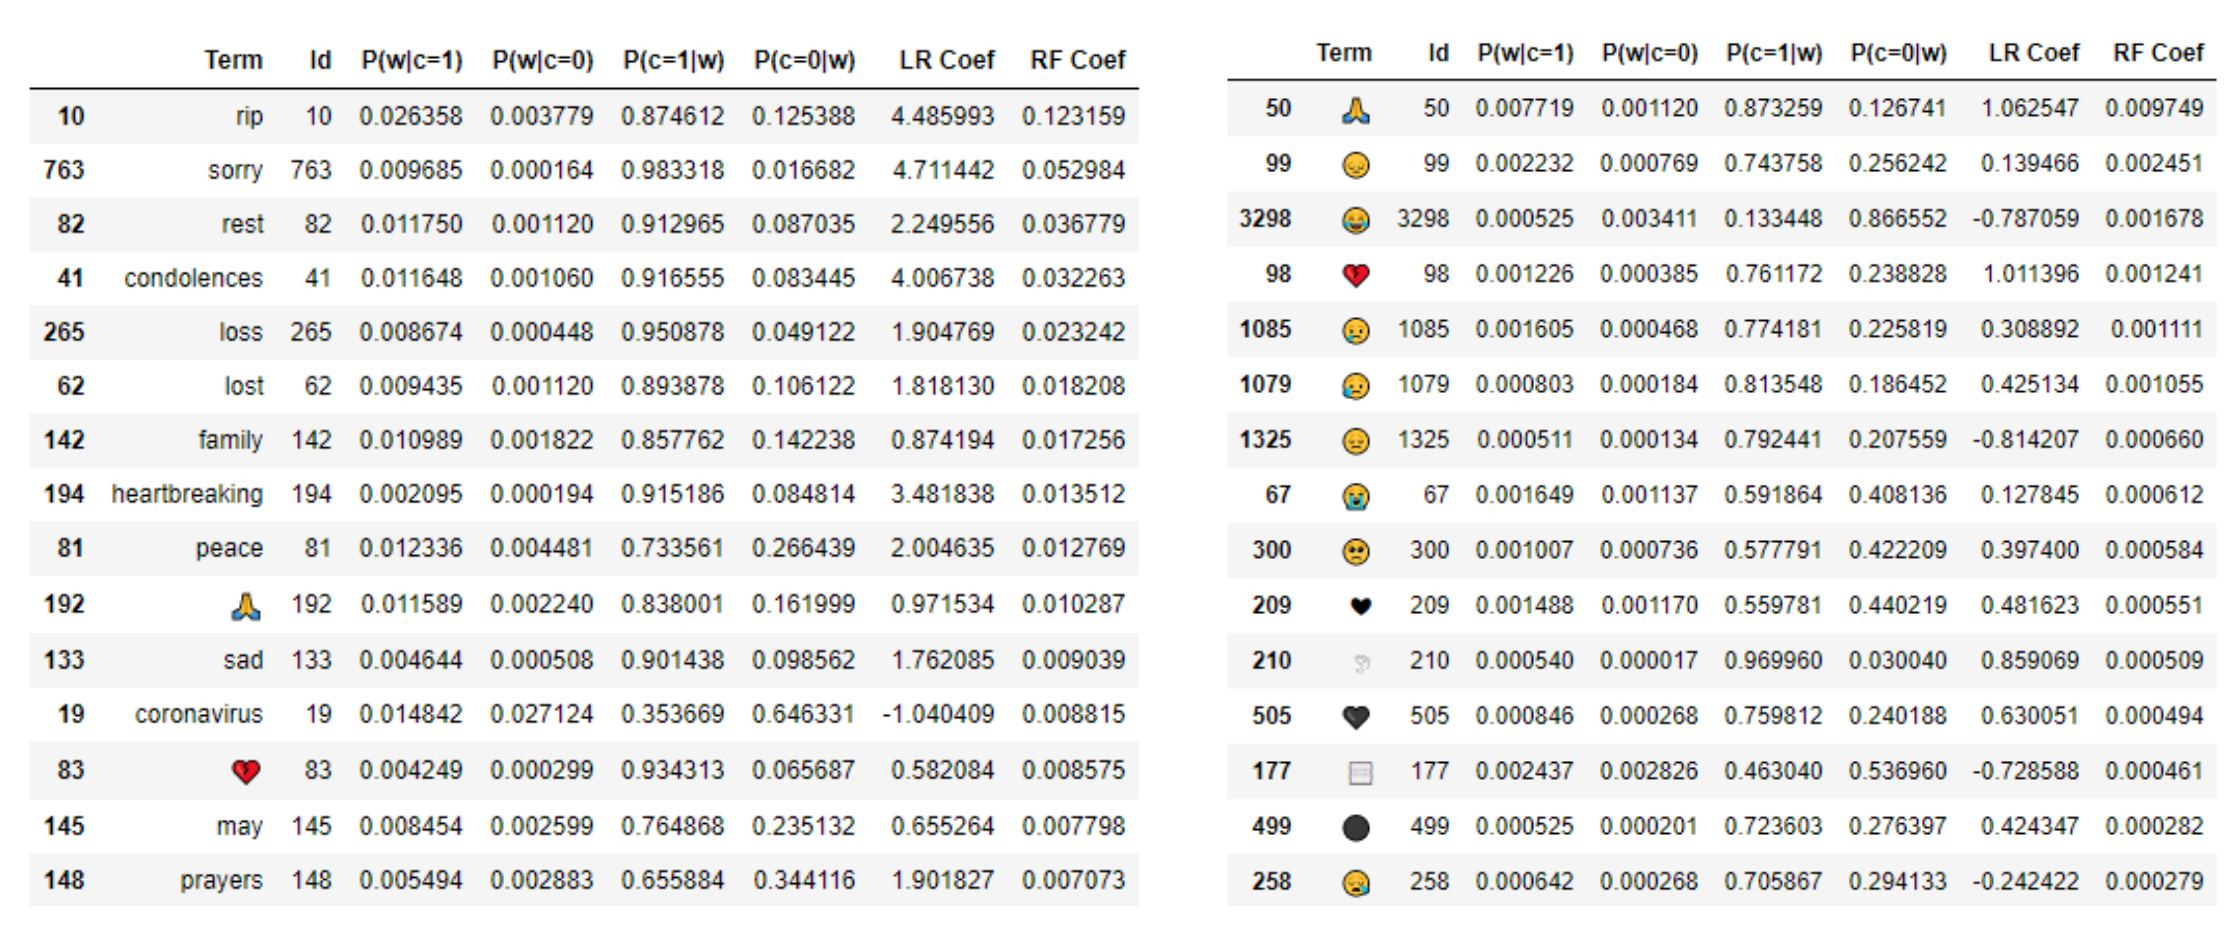
\includegraphics[width=\textwidth]{doc/images/RF_Coef_en.png}
\end{table}

\newpage
\bibliographystyle{unsrt}
\bibliography{biblist.bib}

\end{document}